\chapter{Strategies of carbon conservation and unusual sulphur biogeochemistry Organic Lake}
\label{ch:org}
\acresetall

%---------------------------------------------------------------------------------------------
\section*{Co-authorship Statement}
A version of this chapter has been submitted as:\\

\textbf{Sheree Yau}, Federico M. Lauro, Timothy J. Williams, Matthew Z. DeMaere, Mark V. Brown, John Rich, 
John A.E. Gibson, Ricardo Cavicchioli. 
Strategies of carbon conservation and unusual sulfur biogeochemistry in a hypersaline lake.
\emph{\underline{ISME Journal}}
(submitted), 2013.

Contributions to this manuscript by other researchers is as follows.

Research was designed and manuscript edited by Federico Lauro, John Gibson and Ricardo Cavicchioli.
Sample collection was performed by Federico Lauro, Mark Brown and Ricardo Cavicchioli.
Metagenomic sequence filtering, global assembly and annotation was performed by Matthew DeMaere.
Assistance in intrepretation of functional potential provided by Timothy Williams.

Apart from these contributions, I performed all other data analyses and interpretations.
\newpage

%----------------------------------------------------------------------------------------------

\section{Abstract}
Organic Lake is a shallow, marine-derived hypersaline lake in the Vestfold Hills, Antarctica that has the highest reported concentration of \ac{DMS} in a natural body of water.
To determine the composition and functional potential of the microbial community and learn about the unusual sulphur chemistry in Organic Lake, shotgun metagenomics was performed on size fractionated samples collected along a depth profile.
Eucaryal phytoflagellates were the main photosynthetic organisms.
Bacteria were dominated by the globally distributed heterotrophic taxa \emph{Marinobacter}, \emph{Roseovarius} and \emph{Psychroflexus}.
The dominance of heterotrophic degradation coupled with low fixation potential indicates possible net carbon loss.
However, abundant marker genes for aerobic anoxygenic phototrophy, sulphur oxidation, rhodopsins and CO oxidation were also linked to the dominant heterotrophic bacteria and indicate use of photo- and lithoheterotrophy as mechanisms for conserving organic carbon.
Similarly, a high genetic potential for the recycling of nitrogen compounds likely functions to retain fixed nitrogen in the lake.
\ac{DMSP} lyase genes (\emph{dddD}, \emph{dddL} and \emph{dddP}) were abundant indicating \ac{DMSP} is a significant carbon and energy source.
Unlike marine environments, \ac{DMSP} demethylases (\emph{dmdA}) were less abundant than \ac{DMSP} lyases indicating that \ac{DMSP} cleavage is the likely source of the high \ac{DMS} concentration.
\ac{DMSP} cleavage, photoheterotrophy, lithoheterotrophy and nitrogen remineralisation by dominant Organic Lake bacteria are potentially important adaptations to nutrient constraints.
In particular, photo- and lithoheterotrophy reduces the extent of carbon oxidation for energy production allowing more carbon to be used for biosynthetic processes.
The study sheds light on how the microbial community in Organic Lake has adapted to the unique physical and chemical properties of this Antarctic lake environment.

\newpage

%---------------------------------------------------------------------------------------------
\acresetall
\section{Introduction}
%Molecular biology approaches have proven useful for describing the diversity and gene content of microorganisms in Antarctic lakes and for inferring the functional roles of the taxa present \cite{Laybourn-Parry2007}.
%However to date, only a few large scale shotgun metagenome studies have been performed on the Antarctic continent and in the surrounding Southern Ocean \cite{Wilkins2012a}. 
%In the Vestfold Hills, metagenomics and metaproteomics have been used to study Ace Lake (68$^{\circ}$28$'$23.2$''$S, 78$^{\circ}$11$'$20.8$''$E) \cite{Ng2010a, Lauro2011} and Organic Lake (68$^{\circ}$27$'$23.4$''$S, 78$^{\circ}$11$'$22.6$''$E) \cite{Yau2010}.
%For Ace Lake, a comprehensive assessment of the community structure, biogeochemical fluxes and responses to resource limitation have been described \cite{Lauro2011}.
%The metabolism of abundant green sulphur bacteria \cite{Ng2010a} was found to play a central role in nutrient cycling and a mathematical model was developed that showed its dominance was dependent on synchronicity with the polar light cycle leading to absence of phage predation \cite{Lauro2011}.
%For Organic Lake, a member of the virophage virus family was discovered that potentially regulates microbial loop dynamics \cite{Yau2011}. 
%The Organic Lake virophage likely depends on phycodnaviruses (algal viruses) and it was predicted that the virophage would reduce infective phycodnaviruses leading to an increased frequency of algal blooms and thus carbon flux \cite{Yau2011}.
%Virophage sequences were also identified in a range of aquatic metagenomes revealing that they are likely to play ecologically important roles in many aquatic systems \cite{Yau2011}. 
%These studies on Ace and Organic lakes both used shotgun metagenomics and illustrate the value of adopting a metagenomics approach for learning about microbial ecology in Antarctic environments.
Due to the polar light cycle, phototrophic growth in Antarctic environments is relatively high in summer and negligible in winter \cite{Laybourn-Parry2005} and requires microbial life to survive under long periods under a scarcity of resources.
To overcome this limitation, Eucaryotic phytoflagellates in Ace Lake engage in carbon mixotrophy by grazing on bacterioplankton to supplement their carbon requirements in the winter \cite{Laybourn-Parry2005}.
Marine heterotrophic bacteria are known to be similarly resourceful by exploiting light energy through photoheterotrophy that includes \ac{AAnP} or via use of rhodopsins, or lithoheterotrophy such as oxidation of carbon monoxide \cite{Moran2007b}.
Heterotrophic bacteria that can harness energy sources apart from organic carbon can direct a greater proportion of carbon towards growth, which serves to conserve fixed carbon within a closed systems \cite{Moran2007b}. 

Organic Lake is shallow ($\sim$7 m) and has variable surface water temperatures ($-$14 to $+$15$^{\circ}$C) while remaining sub-zero throughout most of its depth \cite{Franzmann1987b, Gibson1991, Roberts1993b, Gibson1999}.
The salt and marine biota in the lake originate from seawater that was trapped in a basin $\sim$3,000 BP \cite{Zwartz1998, Bird1991}. 
The bottom waters of Organic Lake are unusual due to the absence of hydrogen sulphide and the high concentration of the volatile gas \ac{DMS} \cite{Deprez1986, Franzmann1987b, Gibson1991, Roberts1993a, Roberts1993b}. 
Concentrations of \ac{DMS} as high as 5,000 nM have been recorded in Organic Lake \cite{Gibson1991}, 100 times the maximum concentration recorded from seawater in the adjacent Prydz Bay and at least 1,000 times that of the open Southern Ocean \cite{Curran1998}.
More than forty years ago atmospheric \ac{DMS} was proposed to have a regulatory effect on global cloud cover as it is a precursor of cloud condensation nuclei \cite{Lovelock1972, Charlson1987}.
However, the first enzymes involved in \ac{DMS} production were only identified in the last six years \cite{Todd2007}.
Rapid progress has been made in this short period and the pathways and organisms involved in \ac{DMS} transformations have been extensively reviewed \cite{Johnston2008, Schafer2010, Curson2011b, Reisch2011b, Moran2012}. 

The main source of \ac{DMS} in the marine environment is from the breakdown of \ac{DMSP}. 
Eucaryal phytoplankton, in particular diatoms, dinoflagellates and haptophytes, produce large quantities of \ac{DMSP}, an organo-sulphur compound that is thought to function principally as an osmolyte. 
\ac{DMSP} is released due to cell lysis, grazing or leakage and follows two known fates: \ac{DMSP} cleavage by \ac{DMSP} lyases (DddD, -L, -P, -Q, -W and -Y) or demethylation by \ac{DMSP} demethylase (DmdA).
 Both pathways are associated with diverse microorganisms that can utilize \ac{DMSP} as a sole carbon and energy source. 
However, it is only the cleavage pathway that releases volatile \ac{DMS} that can lead to sulphur loss through ventilation to the atmosphere.
The very high levels of \ac{DMS} in Organic Lake make it an ideal system for identifying the microorganisms and the processes involved in \ac{DMS} accumulation. 

The previous Organic Lake metagenomic study examined viruses from the 0.1 \textmu{}m fraction of surface water that was collected from Organic Lake in December 2006, and November and December 2008 \cite{Yau2011} (Chapter \ref{ch:olv}). 
In the present study we focused on the cellular population rather than viruses. 
Our study determined the composition and functional potential of Organic Lake microbiota and, in conjunction with historic and contemporary physico-chemical data, generated an integrative understanding of the whole lake ecosystem. 
%------------------------------------------------------------------------------------------

\section{Materials and methods}
\subsection{Characteristics of the lake and sample collection}
The water level of Organic Lake was measured by surveying as $+$1.886 m relative to the survey mark (NMV / S / 53) located at 68$^{\circ}$27$'$23.4$''$S, 78$^{\circ}$11$'$22.6$''$E.
Water was collected from Organic Lake on 10 November 2008 through a 30 cm hole in the 0.8 m thick ice cover above the deepest point in the lake. 
The sampling hole was established at 68$^{\circ}$27$'$22.2$''$S, 78$^{\circ}$11$'$23.9$''$E) following bathymetry measurements constructed on a metric grid. 
Samples were collected for metagenomics, microscopy and chemical analyses at 1.7, 4.2, 5.7, 6.5 and 6.7 m depths (maximum lake depth 6.8 m).

For metagenomics, lake water was passed through a 20 \textmu{}m pore size pre-filter, and microbial biomass captured by sequential filtration onto 3.0 \textmu{}m, 0.8 \textmu{}m and 0.1 \textmu{}m pore size 293 mm polyethersulfone membrane filters, and samples immediately preserved in buffer and cryogenically frozen in liquid nitrogen, as described previously \cite{Ng2010a, Lauro2011}. 
Between 1--2 L of lake water was sufficient to saturate the holding capacity of the filters. 
\textsc{DNA} was extracted from the filters, samples sequenced using the Roche GS-FLX titanium sequencer, and reads processed to remove low quality bases, assembled and annotated, as previously described \cite{Ng2010a, Lauro2011}. 
A summary of the 2.4 Gbp of metagenomic data is provided in \tabreft{tab:metag}.
\begin{table}
\footnotesize
\caption[Summary of metagenomic data for Organic Lake profile]{Summary of metagenomic data for Organic Lake November 2008 profile. scf, scaffolds.}
\label{tab:metag}
\smallskip
\begin{tabularx}{\textwidth}{p{0.7cm}p{0.8cm}p{0.6cm}p{1.2cm}p{1.8cm}Xp{1.8cm}X}
\toprule
\textbf{ID} & \textbf{Depth (m)} & \textbf{Size (\textmu{}m)} & \textbf{Trimmed reads} & \textbf{Predicted \acp{ORF} (\%\ac{KEGG} matches)} & \textbf{Scaffolds (reads)} & \textbf{Scaffolds $>$10 kbp (reads)} & \textbf{Annotated scf \acp{ORF} (total scf \acp{ORF})} \\
\midrule
GS374 & 1.7 & 0.1 & 494,573 & 533,468 (31) & 4,318 (63,194) & 5 (771) & 33,262 (83,684)\\
 &  & 0.8 & 472,635 & 470,949 (52) & 4,161 (126,519) & 68 (17,061) & 37,857 (63,140)\\
 &  & 3.0 & 158,121 & 158,573 (50) & 2,584 (39,591) & 4 (520) & 18,126 (28,425)\\
GS375 & 4.2 & 0.1 & 541,962 & 556,791 (30) & 4,899 (80,316) & 2 (232) & 35,318 (87,631)\\
 &  & 0.8 & 472,570 & 492,130 (53) & 5,104 (127,243) & 80 (18,461) & 42,508 (68,366)\\
 &  & 3.0 & 321,112 & 324,365 (56) & 3,983 (98,102) & 69 (14,713) & 30,938 (51,452)\\
GS376 & 5.7 & 0.1 & 363,280 & 387,528 (25) & 2,342 (39,422) & 6 (1,801) & 21,798 (61,595)\\
 &  & 0.8 & 484,635 & 448,373 (59) & 6,820 (152,646) & 134 (29,903) & 47,846 (73, 282)\\
 &  & 3.0 & 290,428 & 292,358 (51) & 3,571 (77,277) & 58 (10,231) & 28,199 (48,910)\\
GS377 & 6.5 & 0.1 & 497,363 & 572,892 (29) & 5,029 (80,520) & 14 (2,711) & 36,685 (92,420)\\
 &  & 0.8 & 465,381 & 454,018 (51) & 4,202 (129,193) & 57 (17,004) & 43,852 (70,382)\\
 &  & 3.0 & 187,045 & 211,354 (59) & 2,100 (60,636) & 51 (9,321) & 20,713 (33,497)\\
GS378 & 6.7 & 0.1 & 516,870 & 586,375 (26) & 3,694 (58,618) & 14 (3,422) & 33,243 (96,334)\\
 &  & 0.8 & 548,253 & 626,115 (57) & 6,957 (161,202) & 136 (32,889) & 56,452 (88,738)\\
 &  & 3.0 & 202,310 & 219,992 (58) & 2,304 (66,389) & 57 (11,167) & 22,786 (35,034)\\
\bottomrule
\end{tabularx}
\end{table}


\subsection{Physical and chemical analyses}
An \emph{in situ} profile of pH, conductivity, turbidity, \ac{DO} and pressure was measured using a submersible probe (\textsc{YSI} sonde model V6600). 
A temperature profile was measured using a maximum-minimum mercury thermometer as the \textsc{YSI} probe did not have a capacity to record temperature below $-$10$^{\circ}$C. 
The 5.7 m sample corresponded to the turbidity maximum and the 6.5 m sample to the turbidity minimum. 
Conductivity at \emph{in situ} temperature was converted to conductivity at 15$^{\circ}$C as described previously \cite{Gibson1999}. 
The adjusted conductivity brings the temperature to within a range suitable for estimating practical salinity using the formula of \citet{Fofonoff1983}. 
Salinity was likely to have been underestimated as it is higher than the range (2--42) for which the conductivity--salinity relation holds. 
However, the relative difference in salinity between the samples would be accurate. 

Density was calculated from the \emph{in situ} conductivity and temperature using the equations described by \citet{Gibson1990} and expressed at temperature T as:

$\sigma_T$ = (1000 $-$ density) kg m$^{-3}$

Ammonia, nitrate, nitrite, \ac{TN}, \ac{TDN}, \ac{DRP}, \ac{TP}, \ac{TDP}, \ac{TOC}, \ac{DOC}, \ac{TS} and \ac{TDS} were determined by American Public Health Associations Standard Methods at the Analytical Services, Tasmania. 
Values for dissolved nutrients were measured after filtration through a 0.1 \textmu{}m pore size membrane filter. 
All other nutrients were measured from water collected after filtration through the on-site 20 \textmu{}m pore size pre-filter.
 
Ammonia, nitrate, nitrite, \ac{DRP}, \ac{TN}, \ac{TDN}, \ac{TP} and \ac{TDP} were measured in a Flow Injection Analyser (Lachat Instruments, Colorado, USA). 
\ac{TOC} and \ac{DOC} were determined in the San$++$ Segmented Flow Analyser (Skalar, Breda, Netherlands). 
\ac{TS} and \ac{TDS} were analysed in the 730ES Inductively Coupled Plasma--Atomic Emission Spectrometer (Agilent Technologies, California, USA). 
Principal component analysis \acs{PCA} was performed using the \textsc{Primer} Version 6 statistical package \cite{Clarke2006} on the normalised physical and chemical parameters.

\subsection{Epifluorescence microscopy}
Water samples collected for microscopy were preserved in formaldehyde (1\% v/v). 
Cells and \acs{VLP} were vacuum filtered onto 25 mm polycarbonate 0.015 \textmu{}m pore-size membrane filters (Nuclepore Track-etched, Whatman, GE Healthcare, USA) with a 0.45 \textmu{}m pore-size backing filter. 
The 0.015 \textmu{}m filter was mounted onto a glass slide with ProLong Gold$^{\textregistered}$ anti fade reagent (Invitrogen, Life Technologies, \textsc{NY}, \textsc{USA}) and 2 \textmu{}l (25$\times$ dilution in sterile filtered milliQ water $<$0.015 \textmu{}m) SYBR$^{\textregistered}$ Gold nucleic acid stain (Invitrogen, Life Technologies, \textsc{NY}, \textsc{USA}). 
Prepared slides were visualized in an epifluorescence microscope (Olympus BX61, Hamburg, Germany) under excitation with blue light (460--495 nm, emission 510--550 nm). 
Cell and \ac{VLP} counts were performed on the same filter over 30 random fields of view.

\subsection{Cellular diversity analyses}
Diversity of \emph{Bacteria}, \emph{Archaea} and \emph{Eucarya} was assessed using \ac{SSU} gene sequences. 
Metagenomic reads that matched the 16S and 18S \ac{rRNA} genes were retrieved using \textsc{Metaxa} \cite{Bengtsson2011}. 
Only sequences longer than 200 bp were accepted for downstream analysis. 

The \ac{QIIME} pipeline (version 1.4.0) \cite{Caporaso2010} implementing \textsc{UCLUST}, was used to group \ac{SSU} sequences into \acp{OTU} at 97\% percent identity against the SILVA \ac{SSU} reference database (release 108)
\url{(www.arb-silva.de)}. 
\ac{SSU} sequences that did not cluster with sequences from \textsc{SILVA} were allowed to form new \acp{OTU} (no suppression). 
A representative sequence from each \ac{OTU} was chosen and classified to the genus level using \ac{QIIME} implementing the \ac{RDP} classifier \cite{Wang2007} trained against \textsc{SILVA}. 
Assignments were accepted to the lowest taxonomic rank with bootstrap value $\leq$85\%. 

To allow comparison of the relative abundance of taxa, the number of \ac{SSU} matches per sample filter was normalised to the average number of reads (403,577). 
Statistical analysis on the relative \ac{SSU} abundances was performed using the \textsc{Primer} version 6 package \cite{Clarke2006}. 
The \ac{SSU} counts of each sample filter were aggregated to the genus level and square root transformed to reduce the contribution of highly abundant taxa. 
A resemblance matrix was computed using Bray-Curtis similarity. 
The upper mixed zone (1.7, 4.2 and 5.7 m) and deep zone (6.5 and 6.7 m) samples were designated as separate groups and an analysis of similarity \ac{ANOSIM} performed to test for difference between the two groups. 
BEST analysis was performed with the abiotic variables: conductivity, temperature, turbidity, \ac{DO}, pH, \ac{TOC}, \ac{TN}, \ac{TP}, \ac{TS}, total C:N, total C:P, total N:P, cell counts and \ac{VLP} counts. 
The Bio-Env procedure in \textsc{BEST} looks at all the abiotic variables in combination and finds a subset sufficient to best explain the biotic structure. 
A heat map with bi-clustering dendogram was generated using R and the package `seriation' \cite{Hahsler2008} on the normalised square-root transformed \ac{SSU} counts.

\subsection{Analysis of functional potential}
The relative abundance and taxonomic origin of functional marker genes was used to determine the potential for carbon, nitrogen and sulphur conversions.
The \acp{ORF} were predicted from trimmed metagenomic reads using \textsc{MetaGene} \cite{Noguchi2006} accepting those $>$90 bp in length. 
Open reading frames \acsp{ORF} were translated using the standard bacterial/plastid translation table and compared to protein sequences from the \ac{KEGG} Genes database (release 58) using the \ac{BLAST} \cite{Altschul1990}. 

The \ac{BLAST} output was processed using \ac{KOBAS} version 2.0 \cite{Xie2011} accepting assignments to \ac{KO} groups with e-value $<$1e$-$05 and rank $>$5. 
\ac{KO} groups used as functional markersare listed in Supplementary \tabref{tab:KO_table}. 
Marker enzymes were assigned to taxonomic groups based on the species of origin of the best \ac{KEGG} Genes \textsc{BLASTp} match. 
\begingroup
\footnotesize
\begin{longtable}{p{2.7cm}p{7.5cm}p{1cm}p{1.8cm}}
\caption[List of KEGG orthologs (KO) involved in nutrient cycles that were searched for in the Organic lake metagenome]{Full list of KEGG orthologs involved in carbon, nitrogen and sulphur conversions that were searched for in the Organic lake metagenome.}
\label{tab:KO_table}
\hline
\textbf{Process} & \textbf{Gene} & \textbf{KO} & \textbf{Notes} \tabularnewline
\hline
\endfirsthead
\multicolumn{4}{c}
{\tablename\ \thetable\ -- \textit{Continued from previous page}} \tabularnewline
\hline
\textbf{Process} & \textbf{Gene} & \textbf{KO} & \textbf{Notes} \tabularnewline
\hline
\endhead
\hline \multicolumn{4}{r} {\textit{Continued on next page}} \tabularnewline
\endfoot
\hline
\endlastfoot
 C fixation & ribulose-bisphosphate carboxylase large (\emph{cbbL}) & K01601  & Calvin cycle \tabularnewline
 & ribulose-bisphosphate carboxylase small (\emph{cbbS}) & K01602 & Calvin cycle \tabularnewline
 & phosphoribulokinase (\emph{prkB}) & K00855 & Calvin cycle \tabularnewline
 & ATP-citrate lyase alpha (\emph{aclA}) & K15230 & rTCA cycle \tabularnewline
 & ATP-citrate lyase beta (\emph{aclB}) & K15231 & rTCA cycle \tabularnewline
 & citryl-CoA lyase (\emph{ccl}) & K15234 & rTCA cycle \tabularnewline
 & citryl-CoA synthetase (\emph{ccsB}) & K15233 & rTCA cycle \tabularnewline
 & carbon monoxide dehydrogenase/acetyl-CoA synthase alpha (\emph{cdhA}) & K14138 & WL  \tabularnewline
 & carbon monoxide dehydrogenase/acetyl-CoA synthase beta (\emph{cdhB}) & K00190 & WL  \tabularnewline
Respiration & cytochrome C oxidase subunit I (\emph{coxI}) & K02256 & Eucaryotic \tabularnewline
 & cytochrome C oxidase subunit III (\emph{coxIII}) & K02262 & Eucaryotic \tabularnewline
 & cytochrome C oxidase subunit I (\emph{coxA}) & K02274 & Bacterial \tabularnewline
 & cytochrome C oxidase subunit III (\emph{coxC}) & K02276 & Bacterial \tabularnewline
Fermentation & L-lactate dehydrogenase (\emph{ldh}) & K00016 &  \tabularnewline
 & pyruvate:ferredoxinoxidoreductase alpha (\emph{porA}) & K00169 &  \tabularnewline
 & pyruvate:ferredoxinoxidoreductase beta (\emph{porB}) & K00170 &  \tabularnewline
CO oxidation & carbon-monoxide dehydrogenase large (\emph{coxL}) & K03520 &  \tabularnewline
 & carbon-monoxide dehydrogenase medium (\emph{coxM}) & K03519 &  \tabularnewline
 & carbon-monoxide dehydrogenase small (\emph{coxS}) & K03518 &  \tabularnewline
AAnP & photosynthetic reaction center L (\emph{pufL}) & K08928 &  \tabularnewline
 & photosynthetic reaction center M (\emph{pufM}) & K08929 &  \tabularnewline
Methanogenesis & coenzyme M methyl reductase (\emph{mcrB}) & K00401 &  \tabularnewline
 & methyl coenzyme M reductase system & K00400 &  \tabularnewline
CH$_4$ oxidation & soluble methane monooxygenase & K08684 &  \tabularnewline
N fixation & nitrogenase (\emph{anfG}) & K00531 &  \tabularnewline
 & nitrogenase molybdenum-iron protein alpha (\emph{nifD}) & K02586 &  \tabularnewline
 & nitrogenase iron protein (\emph{nifH}) & K02588 &  \tabularnewline
 & nitrogenase  molybdenum-iron protein beta (\emph{nifK}) & K02591 &  \tabularnewline
Denitrification & nitric oxide reductase (\emph{norB}) & K02305 &  \tabularnewline
 & nitric oxide reductase (\emph{norC}) & K02305 &  \tabularnewline
 & nitrous oxide reductase (\emph{nosZ}) & K00376 &  \tabularnewline
DNRA & periplasmic cytochrome c-552 (\emph{nrfA}) & K03385 &  \tabularnewline
N dissimilation & hydroxylamine oxidase (\emph{hao}) & K10535 & \emph{hzo}-like \tabularnewline
N mineralization/ assimilation & glutamate dehydrogenase (\emph{gudB}, \emph{rocG}) & K00260 &  \tabularnewline
 & glutamate dehydrogenase (NAD(P)+) & K00261 &  \tabularnewline
 & glutamate dehydrogenase (\emph{gdhA}) & K00262 &  \tabularnewline
N assimilation & assimilatory nitrate reductase & K00360 &  \tabularnewline
 & assimilatory nitrate reductase (\emph{nasA}) & K00372 &  \tabularnewline
 & assimilatory nitrate reductase (\emph{narG}) & K00367 &  \tabularnewline
 & glutamine synthetase (\emph{glnA}) & K01915 &  \tabularnewline
 & glutamate synthetase (NADPH/NADH)(\emph{gltB}) & K00265 &  \tabularnewline
 & glutamate synthetase (ferredoxin) (\emph{gltS}) & K00284 &  \tabularnewline
Nitrification & ammonia monooxygenase subunit A (\emph{amoA}) & K10944 &  \tabularnewline
 & ammonia monooxygenase subunit B (\emph{amoB}) & K10945 &  \tabularnewline
 & ammonia monooxygenase subunit C (\emph{amoC}) & K10946 &  \tabularnewline
DSR & adenylylsulfatereductase subunit A (\emph{aprA}) & K00394 & SRB related \tabularnewline
 & adenylylsulfatereductase subunit B (\emph{aprB}) & K00395 & SRB related \tabularnewline\
 & sulfite reductase (\emph{dsrA}) & K11180 & SRB related \tabularnewline
 & sulfite reductase (\emph{dsrB}) & K11181 & SRB related \tabularnewline
ASR & adenylyl sulfate kinase (\emph{cysC}) & K00860 &  \tabularnewline
 & sulfateadenylyltransferase (\emph{cysN}) & K00956 &  \tabularnewline
 & sulfateadenylyltransferase (\emph{cysD}) & K00957 &  \tabularnewline
S mineralisation & cysteine diogenase (\emph{cdoI}) & K00456 &  \tabularnewline
 & thiosulfate/3-Mercaptopyruvate sulfurtransferase (\emph{sseA}) & K01011 &  \tabularnewline
DMSP reduction & anaerobic dimethyl sulfoxidereductase A (\emph{dmsA}) & K07306 &  \tabularnewline
%\hline
\end{longtable}
\endgroup


Marker genes not represented by a \ac{KO} group were assessed by \textsc{BLASTp} queries of marker gene sequences with experimentally confirmed function \tabref{tab:marker_genes} against a database of translated \acp{ORF} predicted from metagenomic reads. 
Matches were accepted if the e-value was $<$1e$-$10 and sequence identity was within the range shared by homologues of the query sequence(s) \tabref{tab:marker_genes}.
\begin{table}
\footnotesize
\caption[List of query functional marker gene sequences]{Functional marker gene sequences used in this study as \ac{BLAST} queries for retrieving homologues in the Organic Lake metagenomes. \%ID, minimum amino acid identity for a match to be considered homologous.}
\label{tab:marker_genes}
\smallskip
\begin{tabularx}{\textwidth}{p{1.6cm}Xp{1.8cm}p{3.5cm}}
\toprule
\textbf{Gene (\%ID)} & \textbf{Organism} & \textbf{Accession} & \textbf{Reference} \\
\midrule
\emph{dddD} (60) & \emph{Marinomonas} sp.MWYL1 & ABR72937.1 &  \citet{Todd2007}\\
 & \emph{Pseudomonas} sp.J465 & ACY01992.1 & \citet{Curson2010}\\
 & \emph{Psychrobacter} sp.J466 & ACY02894.1 & \citet{Curson2010}\\
 & \emph{Halomonas} sp. HTNK1 & ACV84065.1 & \citet{Todd2010}\\
\emph{dddL} (45) & \emph{Sulfitobacter} sp. EE36 & ADK55772.1 & \citet{Curson2008}\\
 & \emph{Rhodobacter sphaeroides} 2.4.1 & ABA77574.1 & \citet{Curson2008}\\
\emph{dddP} (55) & \emph{Roseovarius nubinhibens} ISM & EAP77700.1 & \citet{Todd2009}\\
\emph{dddQ} & \emph{Ruegeria pomeroyi} DSS-3 & AAV94883.1 & \citet{}\\
 & \emph{Roseovarius nubinhibens} ISM & EAP76001.1 & \citet{}\\
 &  & EAP76002.1 & \citet{Todd2011}\\
 & marine metagenome & GOS\_7860946 & \citet{Todd2011}\\
 &  & GOS\_2632696 & \citet{Todd2011}\\
 &  & GOS\_2469775 & \citet{Todd2011}\\
\emph{dddW} & \emph{Ruegeria pomeroyi} DSS-3 & AAV93771.1 & \citet{Todd2012}\\
\emph{dddY} & \emph{Alcaligenes faecalis} & ADT64689.1 & \citet{Curson2011}\\
\emph{dmdA} (50) & \emph{Ruegeria pomeroyi} DSS-3 & AAV95190.1 & \citet{Howard2006}\\
 & \emph{Pelagibacter ubique} HTCC1062 & YP\_265671.1 & \citet{Howard2006}\\
rhodopsin & \emph{Dokdonia donghaensis} MED134 & EAQ40507.1 & \citet{Gomez-Consarnau2007}\\
 & \emph{Vibrio} sp. AND4 & ZP\_02194911.1 & \citet{Gomez-Consarnau2010}\\
 & \emph{Salinibacter ruber} DSM 13855 & YP\_445623.1 & \citet{Balashov2005}\\
\emph{pufL} (45) & \emph{Roseovarius tolerans} & ABK88229.1 & \citet{Labrenz1999}\\
 & \emph{Congregibacter litoralis} KT71 & ZP\_01104363.1 & \citet{Fuchs2006}\\
\emph{pufM} (45) & \emph{Roseovarius tolerans} & ABK88230.1 & \citet{Labrenz1999}\\
 & \emph{Congregibacter litoralis} KT71 & ZP\_01104362.1 & \citet{Fuchs2006}\\
\emph{soxB} (45) & \emph{Sulfurimonas denitrificans} DSM 1251 & YP\_392780.1 & \citet{Sievert2008}\\
 & \emph{Thiomicrospira crunogena} XCL-2 & ABB42141.1 & \citet{Scott2006}\\
\emph{soxA} (45) & \emph{Sulfurimonas denitrificans} DSM 1251 & YP\_392780.1 & \citet{Sievert2008}\\
 & \emph{Thiomicrospira crunogena} XCL-2 & YP\_390871.1 & \citet{Scott2006}\\
\emph{soxC} (45) & \emph{Sulfurimonas denitrificans} DSM 1251 & YP\_394569.1 & \citet{Sievert2008}\\
 & \emph{Thiomicrospira crunogena} XCL-2 & YP\_390427.1 & \citet{Scott2006}\\
\emph{soxD} (45) & \emph{Sulfurimonas denitrificans} DSM 1251 & YP\_394568.1 & \citet{Sievert2008}\\
 & \emph{Thiomicrospira crunogena} XCL-2 & YP\_390427.1 & \citet{Scott2006}\\
\emph{sqr} (60)  & \emph{Sulfurimonas denitrificans} DSM 1251 & ABB43898.1 & \citet{Sievert2008}\\
\emph{recA} & \emph{Escherichia coli} K12 & P0A7G6.2 & \citet{Howard2008}\\
\bottomrule
\end{tabularx}
\end{table}

Matches to marker genes were normalised to 100 Mbp per sample and counted. 
Normalised frequencies of markers from the same pathway were averaged and those from different pathways were summed. 

The same marker genes and \ac{BLAST} procedure was used to compare the \ac{DMSP} catabolism and photoheterotrophy potential of Organic Lake with nearby Ace Lake \cite{Lauro2011}, \ac{SO} \cite{Wilkins2012b} and \ac{GOS} metagenomes \cite{Rusch2007}. 
Counts of single copy gene \emph{recA} were also determined to estimate the percentage of genomes containing each marker gene (percentage of marker genes relative to \emph{recA}). 
Matches to \emph{recA} were accepted with e-value $<$1e$-$20 according to the cut-off established by \citet{Howard2008}. 
For \ac{GOS} samples, the \ac{BLAST} database was generated from peptide sequences retrieved from \ac{CAMERA} (camera.calit2.net) while the other \ac{BLAST} databases were produced as for Organic Lake. 
The total number of trimmed base pairs for \ac{GOS} samples was estimated by multiplying the number of reads from each sample by the average read length (822 bp) \cite{Rusch2007}. 

Marker gene sequences for phylogenetic analysis were clustered using the \textsc{CD-HIT} web server \cite{Huang2010} at 90\% global amino acid identity. 
A representative sequence from the clusters that resided within a desired conserved region and homologues from cultured strainswere used in phylogenetic analyses performed in \ac{MEGA} 5.05 \cite{Tamura2011} implementing \textsc{MUSCLE} with default parameters (gap opening penalty: $-$2.9, gap extension penalty: 0). 
Neighbor-joining was used to compute the phylogenies with a Poisson substitution model, uniform rates of change and complete deletion of alignment gaps. 
Node support was tested with bootstrap analysis (500 replicates). 

%-----------------------------------------------------------------------------------------


\section{Results and discussion}

\subsection{Abiotic properties and water column structure}
\emph{In situ} physico-chemical profiles \figref{fig:probe_profiles} measured over the deepest point in the lake \figref{fig:bathymetry} determined the existence of two zones: an upper mixed zone above 5.7 m and a suboxic deep zone below 5.7 m \figref{fig:vert_struc}.
\begin{figure}
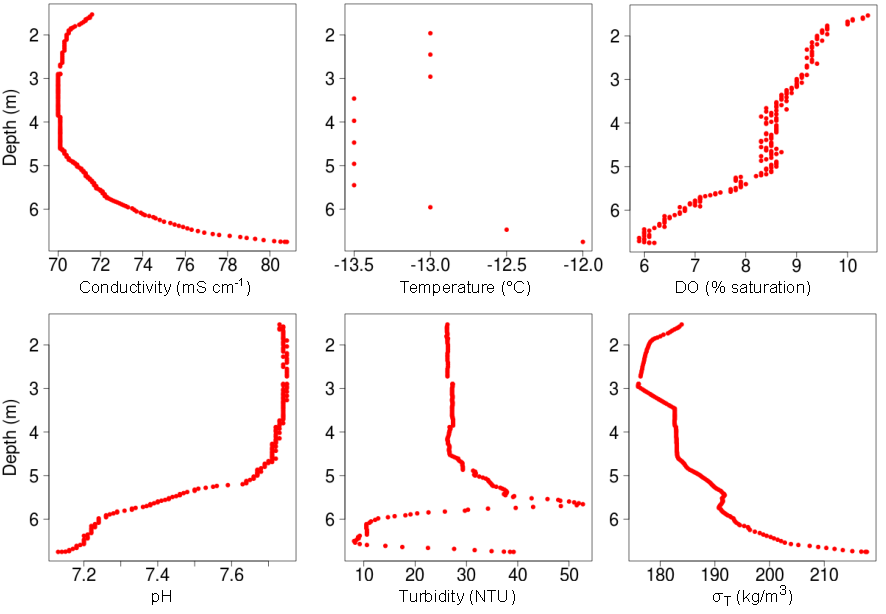
\includegraphics{orglake_figures/probe_profiles.pdf}
\caption[Vertical profiles of \emph{in situ} Organic Lake abiotic parameters]{Vertical profiles of \emph{in situ} Organic Lake abiotic parameters measured at the deepest point in the lake on 9 November 2008. $\sigma_{T} =$ (1000 $-$ density) was calculated from temperature and conductivity}
\label{fig:probe_profiles}

\end{figure}

\begin{figure}
\centering
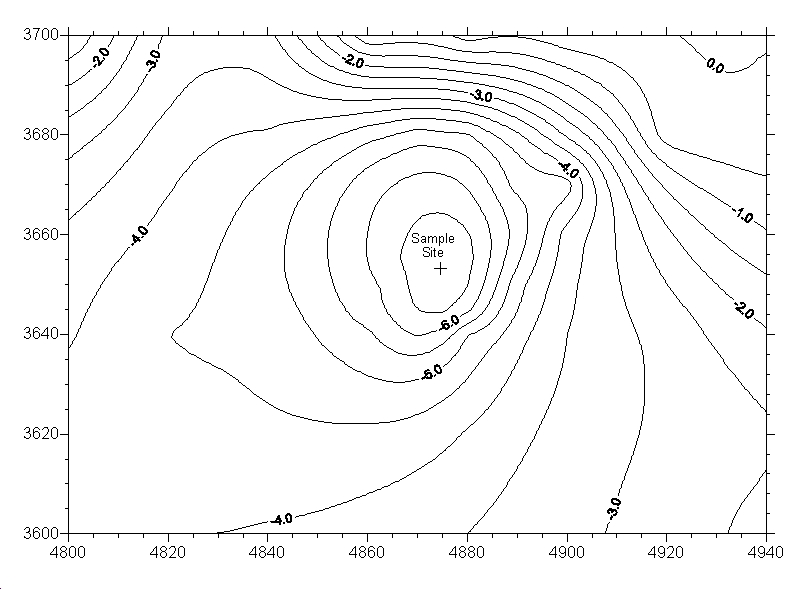
\includegraphics[width=100mm]{orglake_figures/bathymetry.jpg}
\caption[Bathymetry of Organic Lake]{Bathymetry of Organic Lake 9 November 2008. Eastings and northings shown are abbreviated metric map grid co-ordinates.}
\label{fig:bathymetry}

\end{figure}

\begin{figure}
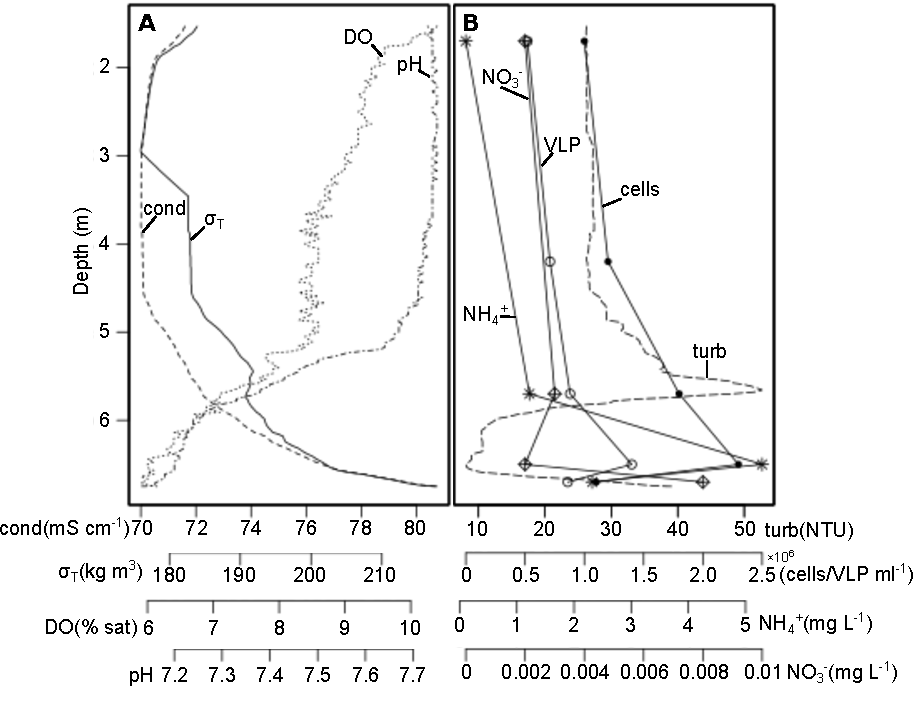
\includegraphics[width=\textwidth]{orglake_figures/vert_struc.pdf}
\caption[Vertical structure of Organic Lake]{Vertical structure of Organic Lake. (\textbf{A}) Parameters that varied unimodally with depth showed two zones: an aerobic mixed zone above 5.7 m and a denser suboxic zone below. (\textbf{B}) Additional factors that revealed stratification within the deep zone. The peak in concentration at 6.5 m for ammonia was also observed for all other nutrients assayed except nitrate and nitrite, see \tabref{tab:physico-chem} for these values. $\sigma_{T} =$ (1000 $-$ density); cond, conductivity; \textsc{DO}, dissolved oxygen; turb, turbidity.}
\label{fig:vert_struc}

\end{figure}

The separation of the two zones was indicated by a pycnocline and oxycline starting at 5.7 m. 
The pH also decreased with \ac{DO}, likely due to fermentation products such as acetic, formic and lactic acids that have been reported in the bottom waters \cite{Franzmann1987b, Gibson1994}.
The deep zone was not completely anoxic \figref{fig:probe_profiles}.
Oxygen may be episodically introduced to bottom waters as a result of currents of cold dense water sinking during surface ice-formation \cite{Ferris1991}.
In comparison to meromictic lakes such as Ace Lake that have strong pycnoclines and a steep salt gradient in the anoxic zone, Organic Lake is shallow and has relatively weak stratification \cite{Gibson1999}. 


Samples were collected from the upper mixed (1.7, 4.2 and 5.7 m) and deep (6.5 m and 6.7 m) zones. 
All nutrients, except for nitrate and nitrite reached maximum concentrations at 6.5 m \tabref{tab:physico-chem} suggestive of a layer of high biological activity above the lake bottom. 
\begin{table}
\footnotesize
\caption[Physico-chemical properties of Organic Lake 2008 vertical profile]{Physico-chemical properties, cell counts and \ac{VLP} counts of Organic Lake 2008 samples from a vertical profile. ND, data not determined.}
\label{tab:physico-chem}
\smallskip
\begin{tabularx}{\textwidth}{p{2.6cm}XXXXX}
\toprule
 & \multicolumn{5}{c}{\textbf{sample depths (m)}}\\
 & \textbf{1.7} & \textbf{4.2} & \textbf{5.7} & \textbf{6.5} & \textbf{6.7}\\
\midrule
ammonia (mg l$^{-1}$) & 0.108 & ND & 1.22 & 5.29 & 2.32 \\
nitrate (mg l$^{-1}$) & $<$0.002 & ND & 0.003 & $<$0.002 & 0.008 \\
nitrite (mg l$^{-1}$) & $<$0.002 & ND & $<$0.002 & 0.010 & 0.010 \\
\ac{DRP} (mg l$^{-1}$) & 0.08 & ND & 0.10 & 0.20 & 0.18 \\
\ac{TOC} (mg l$^{-1}$) & 88 & 87 & 110 & 170 & 130 \\
\ac{DOC} (mg l$^{-1}$) & 69 & ND & 97 & 150 & 120 \\
\ac{TN} (mg l$^{-1}$) & 7.70 & 7.50 & 11 & 24 & 13 \\
\ac{TDN} (mg l$^{-1}$) & 0.112 & ND & 1.225 & 5.302 & 2.338 \\
\ac{TP} (mg l$^{-1}$) & 1.5 & 1.4 & 3.0 & 7.6 & 3.7 \\
\ac{TDP} (mg l$^{-1}$) & 0.509 & ND & 0.805 & 4.5 & 2 \\
\ac{TS} (mg l$^{-1}$) & 1010 & 974 & 1020 & 1410 & 950 \\
\ac{TDS} (mg l$^{-1}$) & 996 & ND & 1250 & 1290 & 995 \\
particulate C:N:P (molar ratios) & 49:7:1 & ND & 15:2:1 & 17:3:1 & 15:1:1 \\
dissolved C:N:P (molar ratios) & 350:20:1 & ND & 311:26:1 & 86:10:1 & 155:13:1 \\
practical salinity & 166 & 166 & 172 & 178 & 186 \\
temperature ($^{\circ}$C) & $-$13 & $-$13.5 & $-$13 & $-$12.5 & $-$12 \\
cells ml$^{-1}$ & 1.0$\pm0.4 \times 10^6$ & 1.2$\pm0.3 \times 10^6$ & 1.8$\pm0.5 \times 10^6$ & 2.3$\pm0.8 \times 10^6$ & 1.1$\pm0.4 \times 10^6$ \\
\ac{VLP} ml$^{-1}$ & 5.2$\pm2.1 \times 10^5$ & 7.1$\pm1.3 \times 10^5$ & 8.8$\pm3.4 \times 10^5$ & 14$\pm3.0 \times 10^5$ & 8.6$\pm3.3 \times 10^5$ \\
\bottomrule
\end{tabularx}
\end{table}

Consistent with this, cell and \ac{VLP} counts were highest at 6.5 m. 
However, turbidity was lowest at this depth demonstrating turbidity was not principally determined by cell density \figref{fig:vert_struc}. 
Microscopy images did not show a shift in cell morphology that could account for the large drop in turbidity \figref{fig:microscopy}, which suggests particulate matter primarily contributed to turbidity readings. 
\begin{figure}
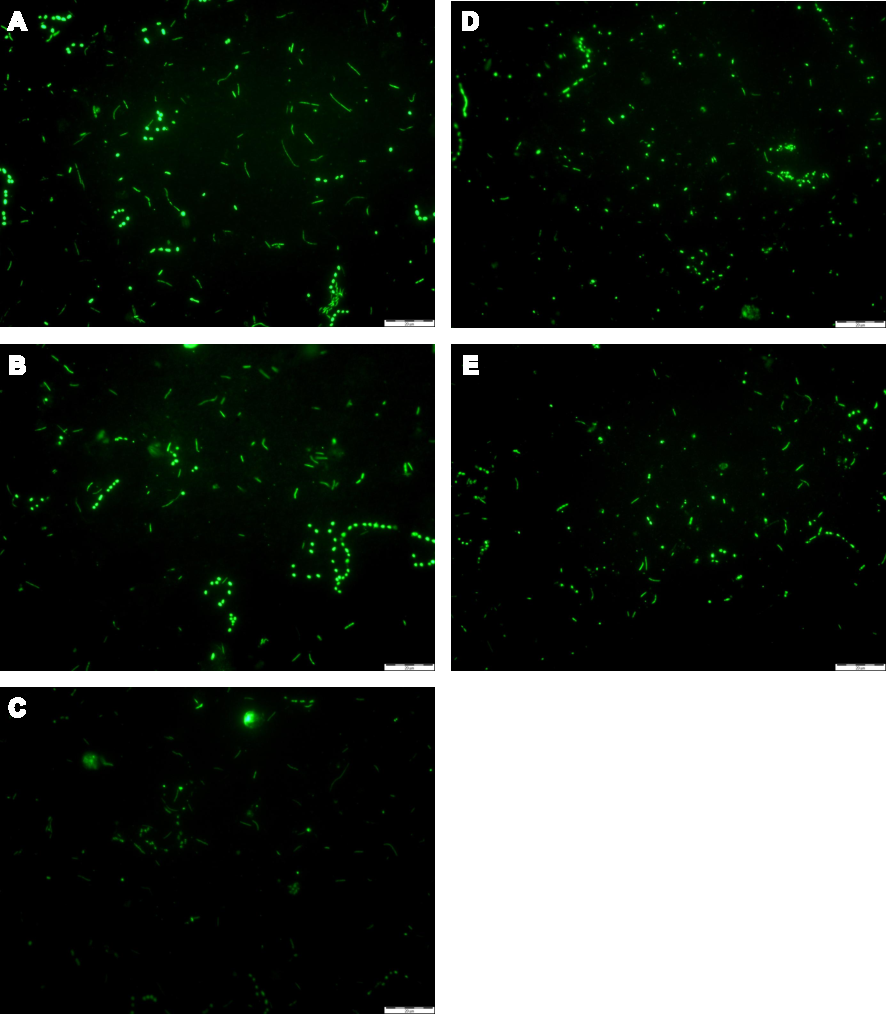
\includegraphics[width=\textwidth]{orglake_figures/microscopy.pdf}
\caption[Epifluorescence microscopy images of Organic Lake microbiota]{Epifluorescence microscopy images of Organic Lake microbiota ($<$20 \textmu{}m) onto 0.015 \textmu{}m polycarbonate membrane and stained with \textsc{SYBR} Gold. (\textbf{A}) 1.7 m, (\textbf{B}) 4.2 m, (\textbf{C}) 5.7 m, (\textbf{D}) 6.5 m, (\textbf{E}) 6.7 m. Scale bar $=$ 20 \textmu{}m. }
\label{fig:microscopy}

\end{figure}

The low turbidity and peak in cell counts and nutrients at the oxycline at 6.5 m may be caused by an active microbial community degrading particulate matter. 
This inference is supported by the report of high concentrations of dissolved organic acids and free amino acids in the deep zone \cite{Gibson1994} as these nutrients are indicative of the breakdown of high molecular weight carbohydrates, lipids and proteins. 
Furthermore, the C:N and C:P ratios throughout the lake were high compared to the Redfield ratio \cite{Redfield1963} except at 6.5 m indicating this was the only depth where dissolved nitrogen and phosphorus were not relatively limited \tabref{tab:physico-chem}.
 
Principal component analysis \acs{PCA} of physico-chemical parameters showed all samples, except the 6.5 m sample, separated with depth along the PC1 axis \figref{fig:pca}.
Accordingly, turbidity, \ac{TS} and cell density were the strongest explanatory variables for the separation of the 6.5 m sample from the other deep sample, indicating that increased activity at 6.5 m was related to breakdown of particulate matter and sulphur chemistry.
\begin{figure}
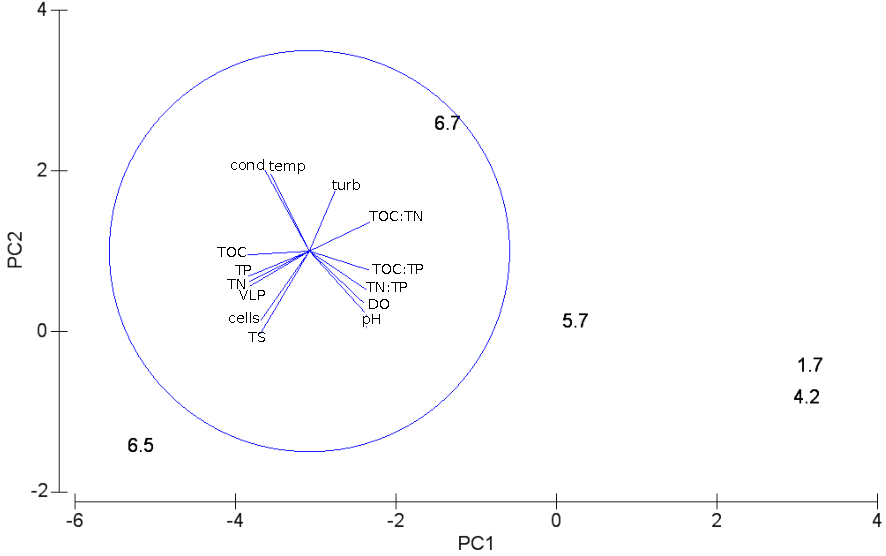
\includegraphics{orglake_figures/pca.pdf}
\caption[PCA analysis of physico-chemical parameters]{PCA analysis of physico-chemical parameters and cell/\ac{VLP} counts of the Organic Lake profile. Data points are the sampling depths 1.7, 4.2, 5.7, 6.5 and 6.7 m. The overlaid vector diagram shows the relative contributions of the variables to explaining the difference between samples. PC1 explained 74.3\% and PC2 explained 14.7\% of the variation between samples. cond, conductivity; temp, temperature; turb, turbidity.}
\label{fig:pca}

\end{figure}
 

\subsection{Overall microbial diversity}
\ac{SSU} genes (3,959 reads) that were retrieved from the metagenome data grouped into 983 \acp{OTU}. 
\acp{OTU} for \emph{Bacteria} comprised 76.2\%, \emph{Eucarya} 16.3\% and 7.5\% of \ac{SSU} sequences could not be classified. 
Only 2 reads, assigned to a deep sea hydrothermal clade of \emph{Halobacteriales} (Supplementary Table S4), were assigned to \emph{Archaea} indicating they were rare in Organic Lake.
 
The most abundant bacterial classes, \emph{Gammaproteobacteria}, \emph{Alphaproteobacteria} and \emph{Flavobacteria}, were represented by \acp{OTU} on all filter sizes at all depths and each consisted of one dominant genus, \emph{Marinobacter}, \emph{Roseovarius} and \emph{Psychroflexus}, respectively \figref{fig:genus_barplots_bact}. 
\begin{figure}
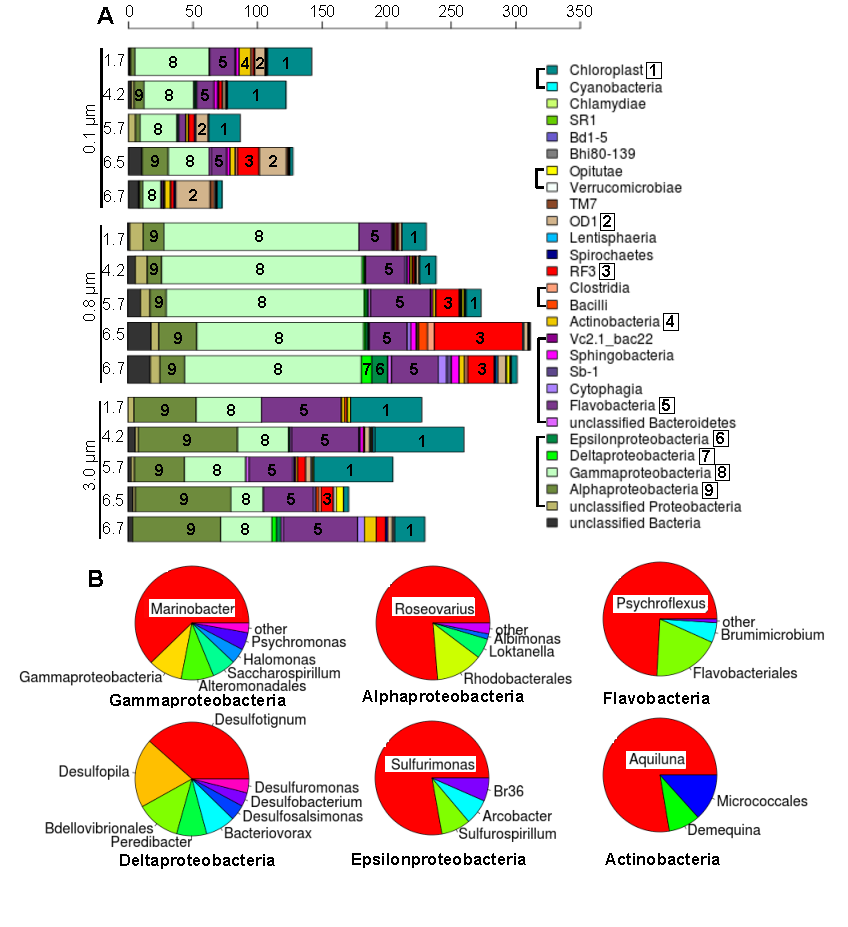
\includegraphics[width=\textwidth]{orglake_figures/genus_barplots3_1.pdf}
\caption[Diversity of \emph{Bacteria} in Organic Lake]{Diversity of (\textbf{A}) \emph{Bacteria} from each size fraction (0.1, 0.8 and 3.0 \textmu{}m) at each sample depth (1.7, 4.2, 5.7, 6.5 and 6.7 m) of Organic Lake aggregated according to class. The x-axis shows counts of \ac{SSU} normalised to average reads acquired per sample filter. Taxa that belong to the same higher rank are shown grouped with a square bracket in the legend. Abundant taxa are labelled in plot with a number that corresponds to the numbered boxes in the legend. (\textbf{B}) Composition of abundant bacterial classes.}
\label{fig:genus_barplots_bact}

\end{figure}

Essentially all \acp{OTU} for \emph{Cyanobacteria}/chloroplasts were classified as chloroplasts \figref{fig:genus_barplots_bact}, except for three reads that could not be assigned to any lower rank (Supplementary Table S4) indicating free-living \emph{Cyanobacteria} were rare or absent. 
\acp{OTU} for moderately abundant bacterial classes were \emph{Actinobacteria}, \emph{Deltaproteobacteria}, \emph{Epsilonproteobacteria}, and candidate divisions OD1 and RF3. 
Lower abundance divisions included \acp{OTU} for \emph{Bacilli}, \emph{Clostridia}, \emph{Spirochaetes}, \emph{Lentisphaeria}, TM7, \emph{Opitutae}, \emph{Verrucomicrobia}, Bhi80-139, Bd1-5, SR1 and \emph{Chlamydiae} \figref{fig:genus_barplots_bact}.

 The dominant eucaryal \acp{OTU} were for photosynthetic \emph{Chlorophyta} (green algae) and \emph{Dictyochophyceae} (silicoflagellate algae) \figref{fig:genus_barplots_euk} principally assigned to the genus \emph{Dunaliella} and the order \emph{Pedinellales}, respectively (Supplementary Table S4). 
Lower abundance eucaryal \acp{OTU} included \emph{Bacillariophyta} (diatoms), \emph{Dinophyceae}, \emph{Fungi} and heterotrophic \emph{Choanoflagellida} and \emph{Ciliophora} (see Supplementary Table S4 for lower taxonomic rank assignments). 
\begin{centering}
\begin{figure}
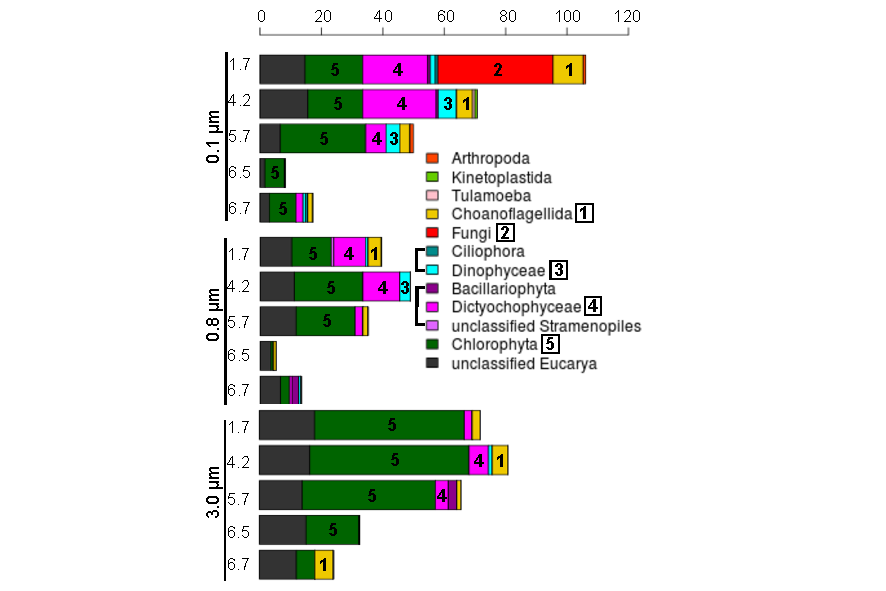
\includegraphics[width=\textwidth]{orglake_figures/genus_barplots3_2.pdf}
\caption[Diversity of \emph{Eucarya} in Organic Lake]{Diversity of \emph{Eucarya} from each size fraction (0.1, 0.8 and 3.0 \textmu{}m) at each sample depth (1.7, 4.2, 5.7, 6.5 and 6.7 m) of Organic Lake aggregated according to class. The x-axis shows counts of \ac{SSU} normalised to average reads acquired per sample filter. Taxa that belong to the same higher rank are shown grouped with a square bracket in the legend. Abundant taxa are labelled in plot with a number that corresponds to the numbered boxes in the legend.}
\label{fig:genus_barplots_euk}

\end{figure}
\end{centering}



\subsection{Variation of microbial composition according to size and depth}
Community composition varied with size fraction and depth. 
This was supported by seriation analysis that showed samples clustered according to size fraction, and those clusters further separated into upper mixed and deep zone groups \figref{fig:heatmap}. 
A significant difference in genus-level composition between the upper mixed and deep zones was supported by \ac{ANOSIM} test (Rho: 0.53, significance: 0.1\%). 
Differential vertical distribution of taxa is consistent with partitioning of ecological functions in the lake and in association with the physical and chemical data, described functional roles of those taxa.
\begin{figure}
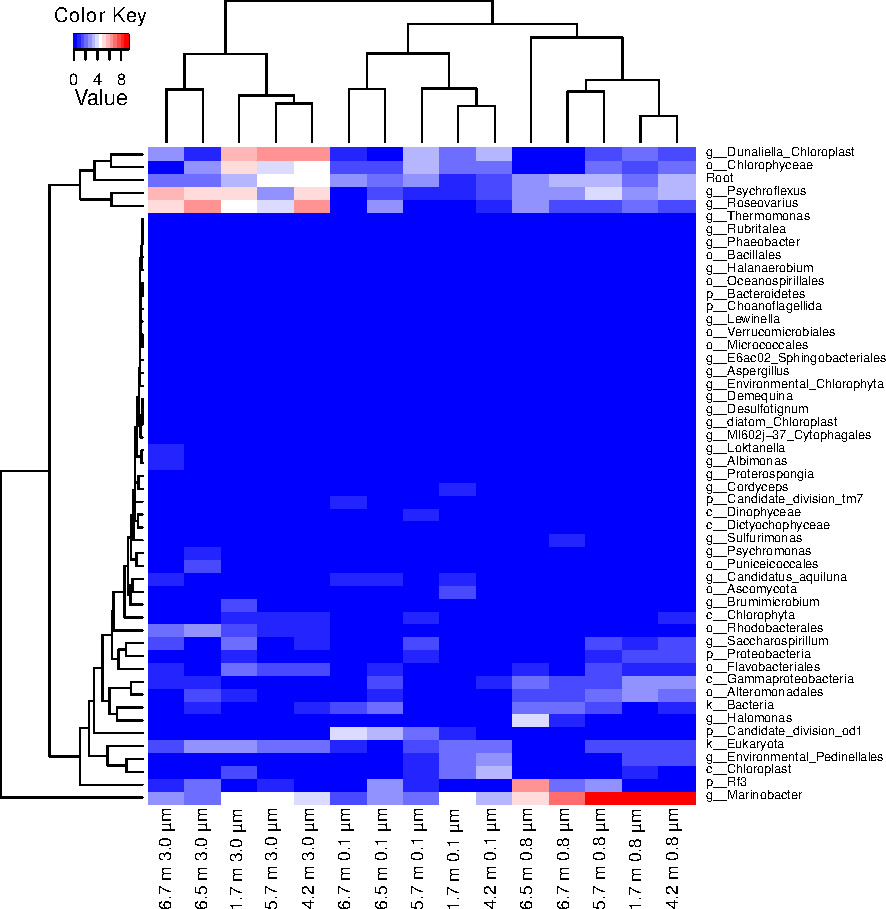
\includegraphics{orglake_figures/heatmap.pdf}
\caption[Heatmap and biclustering plot of the \ac{SSU} gene composition in Organic Lake]{Heatmap and biclustering plot of the \ac{SSU} gene composition in Organic Lake. Samples are shown according to size fraction (0.1, 0.8 and 3.0 \textmu{}m) and depth (1.7, 4.2, 5.7, 6.5 and 6.7 m). \ac{SSU} genes were classified to lowest taxonomic rank that gave bootstrap confidence $>$85\% until the rank of genus. \ac{SSU} gene counts were normalised and square root transformed. Taxa that comprised $<$2\% of the sample were not included.}
\label{fig:heatmap}

\end{figure}


\subsubsection{20--3.0 \textmu{}m fraction community composition}
The upper mixed zone samples had a relatively high \ac{OTU} abundance of \emph{Dunaliella} chloroplasts and chlorophyte algae consistent with large active photosynthetic organisms concentrating near surface light. 
They are likely the main source of primary production in Organic Lake and have previously been reported to be the dominant algae \cite{Franzmann1987b}. 
The \ac{SSU} sequences for these algae at the bottom of the lake are likely to be due to sedimentation of dead cells or resting cysts.

Psychroflexus \acp{OTU} were overrepresented in the surface and 6.7 m samples. 
Consistent with enrichment on the 3.0 \textmu{}m filters, \emph{Psychroflexus} (formerly \emph{Flavobacterium}) \emph{gondwanensis} \cite{Bowman1998} isolated from Organic Lake \cite{Franzmann1987b} had cells 1.5--11.5 \textmu{}m in length \cite{Dobson1991}. 
\emph{Flavobacteria} associate with phytoplankton blooms in the Southern Ocean \cite{Abell2005a, Abell2005b, Williams2012}, and have specialized abilities to degrade polymeric substances from algal exudates and detritus (reviewed in \citet{Kirchman2002}, \cite{Williams2012}). 
It is likely that Organic Lake \emph{Psychroflexus} fills a similar ecological role. 
In support of this, \emph{Psychroflexus} \acp{OTU} cluster with \emph{Dunaliella} chloroplasts in the seriation analysis \figref{fig:heatmap} and \emph{P. gondwanensis} abundance in Organic Lake has been correlated with average hours of sunshine per day indicating population dynamics that is related to summer algal blooms \cite{James1994}. 
The \emph{Psychroflexus} \acp{OTU} in the deep zone are most likely due to sedimentation as \emph{P.gondwanensisis} non-motile and strictly aerobic \cite{Dobson1991}.

\emph{Roseovarius} \acp{OTU} were enriched at 4.2 m and 6.5 m suggesting different ecotypes may be present in the upper mixed zone compared to the deep zone. 
\emph{Roseovarius tolerans}, an isolate from Ekho Lake in the Vestfold Hills, Antarctica has a cell size (1.1--2.2 \textmu{}m; \cite{Labrenz1999}) that would be expected to be captured on the 0.8 \textmu{}m filter. 
The \emph{Roseovarius} captured on the 3 \textmu{}m filter may therefore be a different species, or a strain similar to \emph{R. tolerans} from Ekho Lake that exhibits different growth characteristics (i.e. larger cell size or forms aggregates). 
A strain of this species from Ekho Lake is capable of microaerophilic growth \cite{Labrenz1999}. 
Overrepresentation at 6.5 m may therefore be indicative of growth at that depth rather than sedimentation because sinking cells would be more abundant close to the lake bottom at 6.7 m. 
\emph{Roseovarius} \acp{OTU} cluster with \emph{Dunaliella} chloroplast and \emph{Psychroflexus} \acp{OTU} in the seriation analysis \figref{fig:heatmap}, suggesting that Organic Lake \emph{Roseovarius} may be utilising compounds released from algal-derived particulate matter, or made available by processing of complex organic matter by \emph{Psychroflexus}.
\emph{Roseovarius} is a member of the \emph{Roseobacter} clade, which is inferred to have an opportunistic ecology frequently associated with nutrient-replete plankton aggregates, including by-products of flavobacterial exoenzymatic attack \cite{Moran2007a, Teeling2012}. 
Additionally,the diverse metabolic capabilities of the \emph{Roseobacter} clade include \ac{DMSP} degradation, \ac{AAnP} and CO oxidation (reviewed in \citet{Wagner-Dobler2006}). 
All of these capabilities should facilitate growth in both the upper mixed and deep zones of Organic Lake (see \ref{subs:carbon}).

\subsubsection{3--0.8 \textmu{}m size fraction community composition}
On the 0.8 \textmu{}m filter, \acp{OTU} for \emph{Marinobacter} dominated at all depths except 6.5 m. 
Their capture on this size fraction is consistent with the cell size of isolates (1.2--3 \textmu{}m) \cite{Gauthier1992}. 
The genus is metabolically versatile, which likely permits it to occupy the entire water column. 
\emph{Marinobacter} is heterotrophic and the genus includes hydrocarbon-degrading strains (e.g., \citet{Gauthier1992, Huu1999}, although deep-sea metal-oxidising autotrophs have also been reported \cite{Edwards2003}. 
Some isolates are capable of interacting with diatoms \cite{Gardes2010} and dinoflagellates \cite{Green2006}. 
\emph{Marinobacter} isolates from Antarctic lakes are capable of anaerobic respiration using \ac{DMSO} \cite{Matsuzaki2006} or nitrate \cite{Ward1997}. 
Analysis of functional potential linked to \emph{Marinobacter} revealed additional metabolic capabilities potentially related to its dominance in Organic Lake 
(see Carbon resourcefulness in dominant heterotrophic bacteria and Molecular basis for unusual sulphur chemistry below).%%Add in link

\acp{OTU} for RF3 and Halomonas were overrepresented at 6.5 m, and RF3 sequences were more abundant \figref{fig:heatmap}. 
Their relative abundance in the deep zone indicates a role in microaerophilic processes. 
The majority of RF3 sequences to date are from anaerobic environments including mammalian gut \cite{Tajima1999, Ley2006, Samsudin2011}, sediment \cite{Yanagibayashi1999, Roske2012}, municipal waste leachate \cite{Huang2005}, anaerobic sludge \cite{Chouari2005, Goberna2009, Riviere2009, Tang2011}, a subsurface oil well head \cite{Yamane2011}, and the anaerobic zone of saline lakes \cite{Humayoun2003, Schmidtova2009, Bowman2000a}. 
However, some members have been found in surface waters \cite{Demergasso2008, Xing2009, Yilmaz2012} suggesting not all members are strict anaerobes. 

Several \emph{Halomonas} isolates have been sourced from Organic Lake including two described species \emph{Halomonas subglaciescola} and \emph{H. meridiana}, both of which grow as rods with dimensions consistent with capture on this size fraction \cite{Franzmann1987a, James1990}. 
Despite these isolates being aerobic, \emph{Halomonas} has been reported to be enriched at the oxycline in Organic Lake \cite{James1994} indicating \emph{Halomonas} in the lake plays an ecological role in the suboxic zone. 
This capacity may be linked to the ability of free amino acids and organic acids, which are abundant in the deep zone \cite{Gibson1994}, to stimulate the growth of isolates \cite{Franzmann1987a}.

\subsubsection{0.8--0.1 \textmu{}m size fraction community composition}
A large number of eucaryal sequences were evident in the 0.1 \textmu{}m size fraction. 
The upper zone was overrepresented by \acp{OTU} for \emph{Pedinellales} (silicoflagellate algae) that co-varied with chloroplasts \figref{fig:heatmap}. 
\emph{Pedinellales} have only been detected in Antarctic lakes from molecular studies \cite{Unrein2005, Lauro2011} including Organic Lake \cite{Yau2011} (Chapter \ref{ch:olv}), and light microscopy studies of Antarctic Peninsula freshwater lakes reported 5--8 \textmu{}m diameter cells resembling \emph{Pseudopedinella} \cite{Unrein2005}. 
It is possible that in Organic Lake small (0.8–0.1 \textmu{}m) free-living members or chloroplast-containing cyst forms \cite{Thomsen1988} exist. 
However, without evidence to support this (e.g. by microscopy) it seems more likely that the lake sustains a relatively small number of active photosynthetic cells and the sequences detected arise from cysts or degraded cellular material.

\acp{OTU} for \emph{Candidatus} “Aquiluna”, in the Luna-1 cluster of \emph{Actinobacteria} \cite{Hahn2004, Hahn2009} were most abundant at 1.7 m. 
The genus has small cells ($<$1.2 \textmu{}m; \cite{Hahn2009}, accounting for their concentration on this size fraction. 
Although originally described in freshwater lakes, the same clade was detected in abundance in Ace Lake \cite{Lauro2011} and surface Artic seawater \cite{Kang2012} demonstrating that they play ecological roles in polar saline systems. 
In Ace Lake surface waters they were associated with utilisation of labile carbon and nitrogen substrates \cite{Lauro2011}, and in Organic Lake surface waters they probably perform similar functions. 
The presence of this clade in the deep zone implies a facultative anaerobic lifestyle or sedimented cells. 

The bottom of the water column was distinguished by the presence of \acp{OTU} for candidate divisions OD1 and TM7. 
OD1 was more abundant, and its prevalence on this size fraction is consistent with similar findings for size fractionation of ground water \cite{Miyoshi2005}. 
OD1 is consistently associated with reduced, sulphur-rich, anoxic environments \cite{Harris2004, Elshahed2005}. 
OD1 from Zodletone Spring, Oklahoma, was reported to possess enzymes related to those from anaerobic microorganisms \cite{Elshahed2005}. 
Genomic analyses identified \acp{OTU} for OD1 in the anoxic zone of Ace Lake \cite{Lauro2011}. 
The distribution of OD1 in Organic Lake is consistent with an anaerobic metabolism and potential involvement in sulphur chemistry. 


\subsection{Organic Lake functional potential}
To determine the potential for functional processes in Organic Lake, gene markers for carbon, nitrogen and sulphur conversions  were retrieved from metagenomic reads. 
BEST analysis showed that variation in the population structure was significantly correlated (Rho: 0.519, significance: 0.3\%) with the abiotic parameters, \ac{DO}, temperature, \ac{TS} and \ac{TN}. 
The \ac{DO} gradient has an obvious effect of separating aerobic from anaerobic taxa, and allows oxygen sensitive nitrogen and sulphur processes to occur in the deep zone. 
Functional potential, taxonomic composition and the physico-chemical data were integrated to infer the carbon, nitrogen and sulphur cycles.

\subsection{Carbon resourcefulness in dominant heterotrophic bacteria}
\label{subs:carbon}
In both the upper mixed and deep zones, potential for carbon fixation was much lower than for degradative processes, indicating potential for net carbon loss \figref{fig:c_cycle}.
\begin{figure}
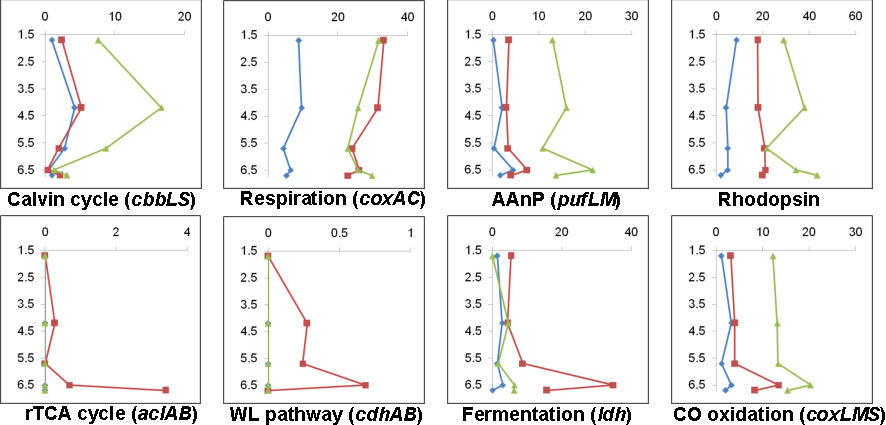
\includegraphics{orglake_figures/c_cycle.pdf}
\caption[Vertical profiles of potential for carbon cycling in Organic Lake]{Vertical profiles of potential for carbon conversions for each size fraction in Organic Lake. The y-axis shows sample depths (m) and the x-axis shows counts of marker genes normalised to 100 Mbp of \textsc{DNA} sequence. The 0.1, 0.8, 3.0 \textmu{}m size fractions are shown as blue, red and green, respectively. Counts for marker genes for the same pathway or enzyme complex were averaged and those from different pathways were summed. For marker gene descriptions see \tabref{tab:KO_table} and \tabref{tab:marker_genes}.}
\label{fig:c_cycle}

\end{figure}
 
Potential for carbon fixation via the oxygen-tolerant Calvin cycle \figref{fig:c_cycle} was originally assessed by presence of the marker genes \ac{RuBisCO} and phosphoribulokinase (\emph{prkB}) \cite{Hugler2011}. 
The majority of \ac{RuBisCO} homologues were related to \emph{Viridiplantae} \tabref{tab:c_cycle_sp} supporting the ecological role of green algae as the principle photosynthetic organisms. 
\begin{table}
\footnotesize
\caption[Contribution of different taxonomic groups to counts of marker genes involved in carbon conversions]{Contribution of different taxonomic groups to counts of marker genes involved in carbon conversions.}
\label{tab:c_cycle_sp}
\smallskip
\begin{tabularx}{\textwidth}{p{3.5cm}XXXXXXXX}
\toprule
\textbf{Taxon} & \rotatebox{45}{\textbf{Calvin cycle}} & \rotatebox{45}{\textbf{\emph{prkB}}} & \rotatebox{45}{\textbf{Respiration}} & \rotatebox{45}{\textbf{Fermentation}} & \rotatebox{45}{\textbf{rTCA}} & \rotatebox{45}{\textbf{WL}} & \rotatebox{45}{\textbf{CO oxidation}} & \rotatebox{45}{\textbf{AAnP}} \\
\midrule
\textbf{\emph{Acidobacteria}} & 0 & 0 & 0.02 & 0 & 0 & 0 & 0 & 0 \\
\textbf{\emph{Actinobacteria}} & 0 & 0 & 0.64 & 0.23 & 0 & 0 & 0.08 & 0 \\
\textbf{\emph{Alphaproteobacteria}} & 0.05 & 0 & 4.84 & 0 & 0 & 0 & \textbf{6.74} & \textbf{6.98} \\
\textbf{\emph{Aquificae}} & 0 & 0 & 0.06 & 0 & 0 & 0 & 0 & 0 \\
\textbf{\emph{Bacteroidetes}} & 0 & 0 & 3.42 & 0 & 0 & 0 & 0 & 0 \\
\textbf{\emph{Betaproteobacteria}} & 0.04 & 0.06 & 0.07 & 0.09 & 0 & 0 & 0.22 & 0 \\
\textbf{\emph{Chlorobi}} & 0 & 0 & 0 & 0 & 0 & 0 & 0 & 0 \\
\textbf{\emph{Chloroflexi}} & 0 & 0 & 0.02 & 0 & 0 & 0 & 0.07 & 0 \\
\textbf{\emph{Chrysiogenetes}} & 0 & 0 & 0 & 0 & 0 & 0  & 0 & 0 \\
\textbf{\emph{Cyanobacteria}} & 0.09 & 0 & 0 & 0 & 0 & 0 & 0 & 0 \\
\textbf{\emph{Deferribacteres}} & 0 & 0 & 0.01 & 0 & 0 & 0 & 0 & 0 \\
\textbf{\emph{Deinococcus-Thermus}} & 0.01 & 0 & 0.02 & 0 & 0 & 0 & 0 & 0 \\
\textbf{\emph{Deltaproteobacteria}} & 0 & 0 & 0.09 & 0 & 0 & \textbf{0.06} & 0.21 & 0 \\
\textbf{\emph{Epsilonproteobacteria}} & 0 & 0 & 0 & 0 & \textbf{0.28} & 0 & 0 & 0 \\
\textbf{\emph{Firmicutes}} & 0.01 & 0 & 0.01 & \textbf{4.90} & 0 & 0.02 & 0.15 & 0 \\
\textbf{\emph{Fornicata}} & 0 & 0 & 0 & 0 & 0 & 0 & 0 & 0 \\
\textbf{\emph{Fusobacteria}} & 0 & 0 & 0 & 0 & 0 & 0 & 0.03 & 0 \\
\textbf{\emph{Gammaproteobacteria}} & 0.05 & \textbf{12.1} & \textbf{9.86} & 1.03 & 0 & 0 & 0.06 & 0.04 \\
\textbf{\emph{Nitrospirae}} & 0 & 0 & 0 & 0 & 0 & 0 & 0 & 0 \\
\textbf{\emph{Planctomycetes}} & 0 & 0 & 0.02 & 0.08 & 0 & 0 & 0 & 0 \\
\textbf{\emph{Spirochaetes}} & 0 & 0 & 0 & 0.03 & 0 & 0 & 0.16 & 0 \\
\textbf{\emph{Thermobaculum}} & 0 & 0 & 0 & 0  & 0  & 0  & 0 & 0 \\
\textbf{\emph{Thermotogae}} & 0.01 & 0 & 0 & 0 & 0 & 0 & 0.17 & 0 \\
\textbf{\emph{Verrucomicrobia}} & 0 & 0 & 0.13 & 0.05 & 0 & 0 & 0 & 0 \\
 &  &  &  &  &  &  &  &  \\
\textbf{\emph{Crenarchaeota}} & 0 & 0 & 0 & 0 & 0 & 0 & 0.01 & 0 \\
\textbf{\emph{Euryarchaeota}} & 0.04 & 0 & 0 & 0 & 0 & 0 & 0 & 0 \\
 &  &  &  &  &  &  &  &  \\
\textbf{\emph{Alveolata}} & 0 & 0 & 0.03 & 0 & 0 & 0 & 0 & 0 \\
\textbf{\emph{Euglenozoa}} & 0 & 0 & 0 & 0 & 0 & 0 & 0 & 0 \\
\textbf{\emph{Opistokonta}} & 0 & 0 & 0.16 & 0 & 0 & 0 & 0 & 0 \\
\textbf{\emph{Rhodophyta}} & 0.16 & 0 & 0.03 & 0 & 0 & 0 & 0 & 0 \\
\textbf{\emph{Strameopiles}} & 0.34 & 0 & 0 & 0 & 0 & 0 & 0 & 0 \\
\textbf{\emph{Viridiplantae}} & \textbf{3.10} & 0.06 & 1.10 & 0 & 0 & 0 & 0 & 0 \\
\bottomrule
\end{tabularx}
\end{table}


\ac{RuBisCO} was only associated with a small proportion of \emph{Gammaproteobacteria} \tabref{tab:c_cycle_sp}, principally from sulphur-oxidising \emph{Thiomicrospira}, indicating some \emph{Gammaproteobacteria} are autotrophs. 
However, the majority of \emph{prkB} matched to \emph{Gammaproteobacteria} \tabref{tab:c_cycle_sp}, predominantly \emph{Marinobacter}. 
Although deep-sea, iron-oxidising autotrophic members of \emph{Marinobacter} have been isolated \cite{Edwards2003}, all genomes reported for \emph{Marinobacter} have \emph{prkB} but lack \ac{RuBisCO} genes. 
Across \emph{Marinobacter} genomes the \emph{prkB} homologue is consistently adjacent to a gene for a putative phosphodiesterase, suggesting that the enzymes expressed by these genes may be involved in a pathway involved in pentose phosphate metabolism unrelated tocarbon fixation. 
Albeit exceptional, this decoupling of \emph{prkB} from \ac{RuBisCO} involved in carbon fixation (forms I and II), also observed in \emph{Ammonifex} \cite{Hugler2011}, undermines the utility of \emph{prkB} as a marker gene for the Calvin cycle within certain groups. 
Thus, there is no evidence for autotrophy in Organic Lake mediated by \emph{Marinobacter}.

Evidence for carbon fixation via the \ac{rTCA} cycle was also indicated \figref{fig:c_cycle}, with genes for ATP citrate lyase (\emph{aclAB}) linked to sulphur-oxidising \emph{Epsilonproteobacteria} \tabref{tab:c_cycle_sp}. 
In general, the \ac{rTCA} cycle is restricted to anaerobic and microaerophilic bacteria \cite{Hugler2011}, which is consistent with the detection of \emph{Epsilonproteobacteria} in the lake bottom where oxygen is lowest, and the microaerophilic/anaerobic metabolisms characteristic of the group \cite{Campbell2006}.
Anaerobic carbon fixation was represented by potential for the \ac{WL} pathway \figref{fig:c_cycle}. 
\ac{WL}-mediated carbon fixation, for which CO dehydrogenase/acetyl-CoA synthaseis the key enzyme, was linked to\emph{Firmicutes} and \emph{Deltaproteobacteria} that are known to grow autotrophically using this pathway \cite{Hugler2011}. 

Potential for carbon loss by via respiration was indicated by an abundance of cytochrome C oxidase genes (\emph{coxAC}) throughout the water column. 
In the deep zone, potential for fermentation was greatest at 6.5 m \figref{fig:c_cycle} and likely the main biological activity that was occurring at that depth. 
Fermentation was indicated by the marker gene lactate dehydrogenase (\emph{ldh}).
These genes were linked to\emph{Firmicutes} \tabref{tab:c_cycle_sp}, which was only present at 6.5 m and represented by the classes \emph{Clostridia} and \emph{Bacilli} \figref{fig:genus_barplots_bact}. 
As the related candidate division RF3 \cite{Tajima1999} also has relatively high abundance in this zone \figref{fig:genus_barplots_bact}
(see 0.8--3.0 \textmu{}m size fraction community composition above), %% add in section link
there is circumstantial evidence that RF3 possesses fermentative metabolism and may therefore play an important ecological role in Organic Lake by degrading high molecular weight compounds to organic acids that other organisms can utilize. 
Assimilation of fermentation products appears to play a greater role in Organic Lake rather than complete anaerobic oxidation involving methanogens or sulphate-reducing bacteria; the former were absent and the latter were present in low abundance \figref{fig:genus_barplots_bact}. 

\emph{Alphaproteobacteria}, predominantly\emph{Roseovarius} \figref{fig:genus_barplots_bact}, were implicated in CO oxidation \tabref{tab:c_cycle_sp}, which is used to generate energy for lithoheterotrophic growth \cite{Moran2007b}, although CO oxidation may also be involved in anaplerotic C fixation \cite{Moran2007b}. 
The CO oxidation capacity was at a maximum at 6.5 m \figref{fig:c_cycle}, and therefore associated with the deep-zone\emph{Roseovarius} ecotype of Organic Lake. 
CO oxidation can function as a strategy to limit oxidation of organic carbon for energy so that a greater proportion can be directed towards biosynthesis \cite{Moran2007b}.

Photosynthesis reaction center genes \emph{pufLM}, involved in photoheterotrophy via \ac{AAnP}, were abundant in Organic Lake (\figreft{fig:c_cycle}, \tabreft{tab:c_cycle_sp}). 
These were linked to the \emph{Roseobacter} clade of \emph{Alphaproteobacteria} \tabref{tab:c_cycle_sp}, major contributors to \ac{AAnP} in ocean surface waters \cite{Beja2002, Moran2007b}. 
This is consistent with the known metabolic potential of \ac{BchlA} producing \emph{Roseovarius tolerans} from Ekho Lake \cite{Labrenz1999}. 
Photoheterotrophy can also be rhodopsin-dependent, with \ac{PR} of marine \emph{Flavobacteria} and \emph{Vibrio} previously linked to light-dependent energy generation to supplement heterotrophic growth, particularly during carbon limitation \cite{Gomez-Consarnau2007, Gomez-Consarnau2010}. 
However, the function(s) of rhodopsins are diverse, and \acp{PR} are also hypothesized to be involved in light or depth sensing \cite{Fuhrman2008}. 

Rhodopsin genes were abundant in Organic Lake \figref{fig:c_cycle}, and were associated with all the dominant Organic Lake aerobic heterotrophic lineages \figref{fig:rhodopsin_tree}. 
\begin{figure}
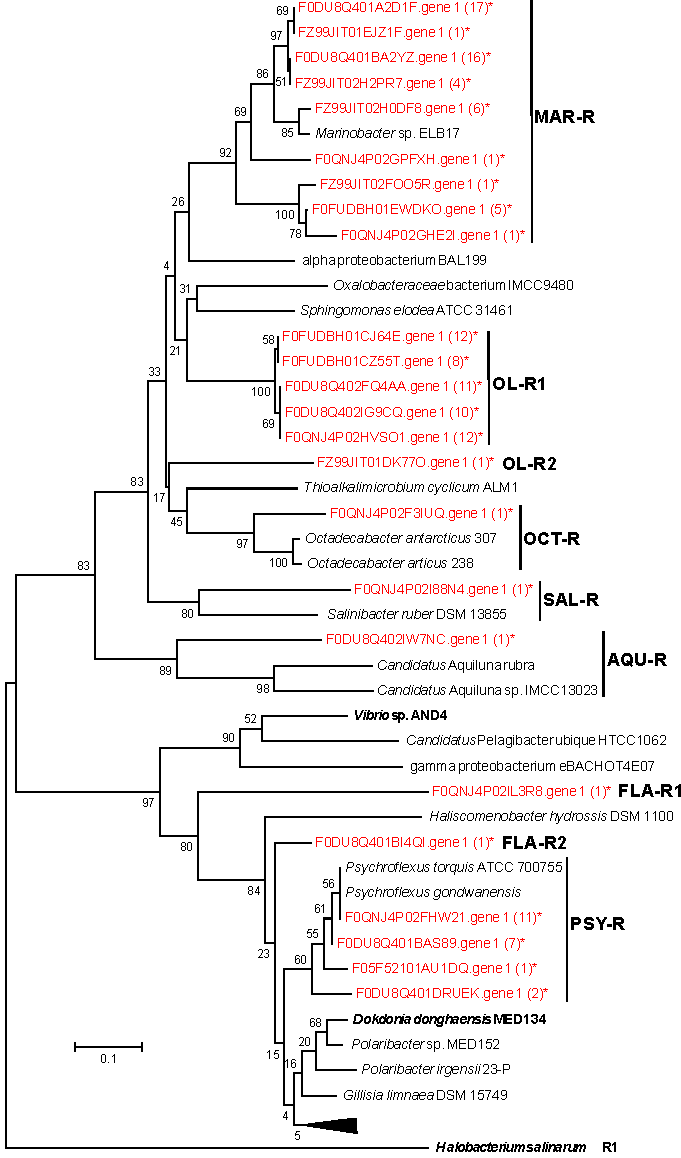
\includegraphics[width=\textwidth]{orglake_figures/rhodopsin_tree.pdf}
\caption[Phylogenetic tree of rhodopsin homologues]{Phylogenetic tree of rhodopsin homologs. \emph{Halobacterium salinarium} R1 halorhodopsin was used as an outgroup. The tree was computed from a 78 amino acid region spanning the motif involved in `spectral tuning' using the neighbour-joining algorithm. Organic Lake sequences from this study are shown in red and marked with an asterisk (*). Numbers in parentheses are counts of sequences that clustered with the Organic Lake homologue shown in the tree with 90\% amino acid identity. Sequences with confirmed activity are shown in bold. Accession numbers from top to bottom are: EAZ99241, EDP63929, EGF32634, ZP\_09955974, AEG32267, EDY76405, EDY88259, YP\_445623, ACN42850, EIC91904, ZP\_02194911, AAZ21446, AAT38609, AEE49633, EAS71907, sequence from John Bowman (personal correspondence), EAQ40507, EAQ40925, EAR12394, EHQ04368 and YP\_001689404.}
\label{fig:rhodopsin_tree}

\end{figure}

Phylogenetic analysis revealed six well-supported Organic Lake rhodopsin groups (Supplementary Figure S6). 
All groups had an L or M residue at position 105 (vs the SAR86 \ac{PR}), denoting tuning to surface green light \cite{Man2003, Gomez-Consarnau2007}, and is characteristic of oceanic coastal samples \cite{Rusch2007}. 
Four of the groups clustered with homologues of genera detected in the lake, namely \emph{Marinobacter}, \emph{Psychroflexus}, \emph{Octadecabacter} and ``\emph{Ca}. Aquiluna'' \figref{fig:rhodopsin_tree} (Table S4). 
Another group (SAL-R group) originates from the sphingobacterium \emph{Salinibacter ruber}, which produces xanthorhodopsin \cite{Balashov2005}; it is therefore likely that Organic Lake \emph{Sphingobacteria} (Supplementary Table S4) were the origin of this rhodopsin group. 
The most abundant group, OL-R1 \figref{fig:rhodopsin_tree} had no close homologues from GenBank, but it was abundant on the 3.0 \textmu{}m fraction and has a distribution suggesting it originates from Organic Lake members of the \emph{Roseobacter} clade \figref{fig:c_cycle}. 
All \acp{ORF} adjacent to OL-R1 rhodopsin containing scaffolds wererelated to \emph{Octadecabacter} further supporting their \emph{Roseobacter} clade provenance \figref{fig:OLR1_scaffolds}. 
Genes downstream of OL-R1 were involved in carotenoid synthesis, indicating OL-R1 is a xanthorhodopsin, occuring as a retinal protein or in a carotenoid complex \cite{Balashov2005}. %%Check, aren't they all retinal?
\begin{figure}
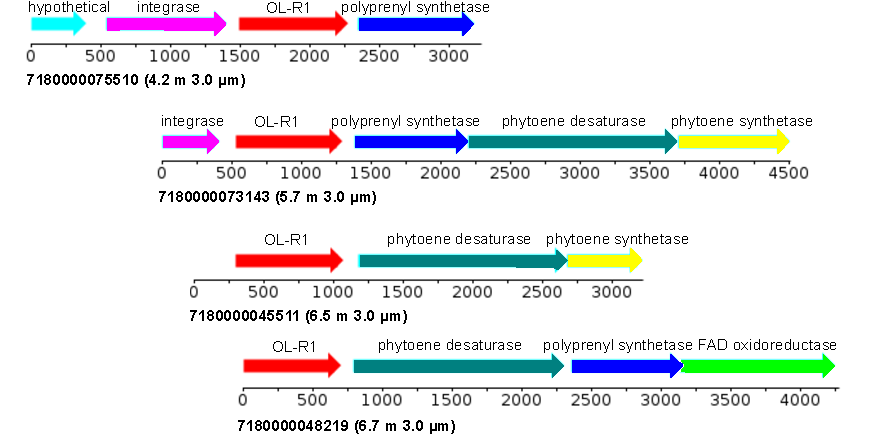
\includegraphics[width=\textwidth]{orglake_figures/OLR1_scaffolds.pdf}
\caption[Maps of OL-R1 rhodopsin-containing scaffolds]{Genomic maps of Organic Lake scaffolds containing the OL-R1 rhodopsin homologue. All genes surrounding OL-R1 had best \ac{BLAST} matches to \emph{Octadecabacter} (\emph{Alphaproteobacteria}) sequences. The scale below shows the number of base pairs. The sample depth and filter from which the scaffold was assembled is shown in parentheses beside the scaffold ID.}
\label{fig:OLR1_scaffolds}

\end{figure}


Photoheterotrophic potential of Organic Lake was compared with other aquatic environments including nearby Ace Lake, \ac{SO} and \ac{GOS} expedition samples. 
The Organic Lake 0.1 \textmu{}m fraction had the lowest rhodopsin counts and percentage of rhodopsin containing cells of all size-matched samples surveyed \tabref{tab:metag_compare}. 
Non-marine \ac{GOS} samples from the 0.1 \textmu{}m fraction have been noted to have lower rhodopsin abundance \cite{Sharma2008}, which was similarly evident from our analysis \tabref{tab:metag_compare}. 
In contrast, the 3.0 \textmu{}m Organic Lake size fractions had higher rhodopsin counts than Ace Lake and comparable counts to the \ac{SO} samples, although the percentage of rhodopsin containing cells was still lower than that of the \ac{SO}. 
The paucity of rhodopsins in the Organic Lake 0.1 \textmu{}m fraction is likely due to the lack of SAR11 clade, which is expected to be the main source of rhodopsin genes in Ace Lake and marine samples. 
This indicates that although Organic Lake has an overall lower frequency of rhodopsin genes compared to sites for which size fraction-matched metagenomes are available, the rhodopsins associated with larger or particle-associated cells are as abundant as in the marine environment.
\begingroup
\footnotesize
\begin{longtable}{p{2.8cm}p{0.5cm}p{1.2cm}p{1cm}p{1cm}p{1.4cm}p{1.4cm}p{1.2cm}p{0.5cm}}
\caption[Counts of genes involved in \ac{DMSP} catabolism and photoheterotrophy in aquatic metagenomes]{Counts of genes involved in \ac{DMSP} catabolism and photoheterotrophy in aquatic metagenomes (normalised to 100 Mbp). 
\% $=$ cells containing marker gene. 
The sample ID for each site is shown in parentheses after the site description. 
Values marked with an asterisk are $>$0 but $<$0.5. 
Counts for the following sites are averages of several samples: Ace Lake mixolimnion (GS232, GS231); Southern Ocean SZ (GS349, GS351--GS353, GS356--GS360); Southern Ocean NZ (GS363, GS346, GS364, GS366–GS368); GOS coastal (GS002--GS004, GS007--GS010, GS012--GS016, GS019, GS021, GS027--GS029, GS034--GS036); GOS open ocean (GS017, GS018, GS022, GS023, GS026, GS037, GS047); GOS estuary (GS006, GS011, GS012). Values shown in bold are the highest for that marker gene. SZ, Southern Zone; NZ, Northern Zone; GOS, Global Ocean Sampling.
}
\label{tab:metag_compare}
\\
\toprule
\textbf{Site} & \textbf{Size (\textmu{}m)} & \textbf{\emph{dddD} (\%)} & \textbf{\emph{dddL} (\%)} & \textbf{\emph{dddP} (\%)} & \textbf{\emph{dmdA} (\%)} & \textbf{Rho. (\%)} & \textbf{\emph{pufLM} (\%)} & \textbf{\emph{recA}} \\
\midrule
\endfirsthead
\multicolumn{9}{c}
{\tablename\ \thetable\ -- \textit{Continued from previous page}} \\
\toprule
\textbf{Site} & \textbf{Size (\textmu{}m)} & \textbf{\emph{dddD} (\%)} & \textbf{\emph{dddL} (\%)} & \textbf{\emph{dddP} (\%)} & \textbf{\emph{dmdA} (\%)} & \textbf{Rho. (\%)} & \textbf{\emph{pufLM} (\%)} & \textbf{\emph{recA}} \\
\midrule
\endhead
\bottomrule \multicolumn{4}{r} {\textit{Continued on next page}} \\
\endfoot
\bottomrule
\endlastfoot
Organic Lake 1.7 m & 0.1 & 2 (9) & 4 (19) & 0 & 0* (2) & 1 (5) & 0* (1) & 21 \\
(GS374) & 0.8 & 10 (36) & 10 (39) & 1 (2) & 2 (7) & 5 (20) & 4 (14) & 26 \\
 & 3.0 & 11 (50) & 5 (21) & 2 (7) & 9 (43) & 12 (57) & 13 (61) & 21 \\
Organic Lake 4.2 m & 0.1 & 5 (34) & 5 (34) & 0 & 1 (10) & 1 (10) & 2 (16) & 14 \\
(GS375) & 0.8 & 15 (54) & 9 (31) & 0 & 2 (6) & 7 (23) & 3 (11) & 28 \\
 & 3.0 & 23 (75) & 2 (8) & 1 (2.5) & 20 (68) & 14 (45) & 16 (53) & 30 \\
Organic Lake 5.7 m & 0.1 & 4 (43) & 1 (7) & 0 & 1 (14) & 2 (21) & 0* (4) & 10 \\
(GS376)  & 0.8 & 6 (20) & 9 (32) & 0 & 2 (7) & 6 (22) & 3 (12) & 29 \\
 & 3.0 & 19 (68) & 3 (12) & 0 & 13 (47) & 6 (21) & 11 (38) & 28 \\
Organic Lake 6.5 m  & 0.1 & 10 (51) & 0* (2) & 0 & 3 (15) & 1 (7) & 4 (22) & 20 \\
(GS377) & 0.8 & 14 (38) & 9 (23) & 1 (2) & 7 (20) & 6 (16) & 7 (20) & 28 \\
 & 3.0 & 42 (106) & 5 (13) & 0 & 20 (52) & 6 (16) & 22 (55) & 29 \\
Organic Lake 6.7 m  & 0.1 & 1 (7) & 0* (4) & 0 & 0 & 1 (7) & 2 (13) & 13 \\
(GS378) & 0.8 & 12 (26) & 8 (17) & 0 & 2 (5) & 8 (16) & 4 (9) & 47 \\
 & 3.0 & 50 (174) & 5 (17) & 4 (13) & 12 (43) & 12 (43) & 14 (48) & 29 \\
Ace Lake & 0.1 & 0* (2) & 0 & 1 (2) & 15 (56) & 15 (53) & 0* (1) & 28 \\
mixolimnion  & 0.8 & 2 (3) & 1 (2) & 0 & 2 (4) & 12 (27) & 3 (12) & 45 \\
 & 3.0 & 0 & 0 & 0* (4) & 0 & 5 (42) & 0 & 11 \\
Newcomb Bay & 0.1 & 6 (14) & 0 & 3 (7) & 50 (111) & 89 (196) & 0 & 45 \\
(GS235)  & 0.8 & 5 (12) & 0 & 0 & 18 (41) & 55 (123) & 0 & 45 \\
 & 3.0 & 0 & 0 & 0 & 2 (17) & 4 (33) & 0 & 11 \\
Southern Ocean & 0.1 & 2 (3) & 0 & 6 (9) & 71 (101) & 98 (139) & 0 & 70 \\
SZ  & 0.8 & 3 (6) & 0* (0*) & 5 (12) & 32 (81) & 43 (108) & 0 & 39 \\
 & 3.0 & 0* (7) & 0 & 0* (4) & 4 (66) & 5 (84) & 0 & 6 \\
Southern Ocean & 0.1 & 0* (1) & 0 & 5 (7) & 124 (159) & 111 (142) & 1 (1) & 78 \\
NZ  & 0.8 & 0* (2) & 0 & 9 (30) & 28 (84) & 35 (107) & 2 (7) & 33 \\
 & 3.0 & 0* (3) & 0 & 1 (9) & 7 (54) & 11 (89) & 0* (4) & 12 \\
GOS coastal & 0.1 & 0* (0) & 0 & 5 (6) & 44 (52) & 74 (87) & 5 (6) & 85 \\
GOS open ocean & 0.1 & 0 & 0 & 7 (8) & 45 (50) & 66 (74) & 5 (5) & 90 \\
GOS estuary & 0.1 & 0 & 0 & 1 (1) & 29 (36) & 61 (77) & 2 (3) & 80 \\
GOS embayment \\(GS005) & 0.1 & 4 (8) & 0 & 6 (12) & 28 (54) & 58 (112) & 3 (6) & 52 \\
GOS Lake Gatun \\(GS020) & 0.1 & 0 & 0 & 0 & 4 (4) & 48 (53) & 2 (2) & 90 \\
GOS fringing reef \\(GS025) & 0.1 & 0 & 0 & 0 & 0 & 7 (39) & 0 & 18 \\
GOS warm seep \\(GS030) & 0.1 & 0 & 0 & 7 (6) & 75 (63) & 83 (69) & 6 (5) & 120 \\
GOS upwelling \\(GS031) & 0.1 & 0 & 0 & 4 (4) & 81 (77) & 81 (76) & 4 (4) & 106 \\
GOS mangrove \\(GS032) & 0.1 & 0 & 0 & 2(3) & 24(34) & 25(36) & 1(1) & 71 \\
GOS Punta Cor-\\morant (GS033) & 0.1 & 0 & 11 (15) & 14 (21) & 4 (6) & 31 (43) & 15 (21) & 72 \\
GOS Rangirora \\Atoll (GS051) & 0.1 & 0 & 0 & 11(15) & 38 (49) & 73 (94) & 3 (4) & 77 \\
\end{longtable}
\endgroup



Counts of \emph{pufLM} genes inthe Organic Lake 0.1 \textmu{}m size fraction were similar to \ac{GOS} sample, except for Punta Cormorant hypersaline lagoon which had the highest \emph{pufLM} counts and percentage of \ac{AAnP} cells \tabref{tab:metag_compare}. 
However, the highest overallcounts of \emph{pufLM} were from the 3.0 \textmu{}m size fraction of Organic Lake, likely due to the high proportion of members of the \emph{Roseobacter} clade. 
Notably, \emph{pufLM} genes were not detected in high abundance in Ace Lake or the \ac{SO} samples, indicating \ac{AAnP} is a unique adaptation in Organic Lake among these polar environments. 
The similarly high abundance of \emph{pufLM} genes in Punta Cormorant hypersaline lagoon indicates \ac{AAnP} may be advantageous in environments with salinity above marine levels.

The contribution of light-driven energy generation processes to the carbon budget is difficult to infer from genetic potential alone. 
For example, the relative abundance of \ac{AAnP} and \ac{PR} genes in Arctic bacteria has been reported to be the same in winter and summer \cite{Cottrell2009}. 
Furthermore, regulation of pigment synthesis is complex; for example, \ac{BchlA} expression in \emph{R. tolerans} occursin the dark but is inhibited by continuous dim light \cite{Labrenz1999}. 
However, it is possible that the apparent negative balance in carbon conversion potential could be ameriolated by photoheterotrophy performed by bacterial groups that are abundant in Organic Lake. 
In particular, the Organic Lake \emph{Psychroflexus} could play a particular role as it has a \ac{PR} related to \emph{Dokdonia}, which was shown to function under carbon-limitation \cite{Gomez-Consarnau2007}.
Furthermore, detection of higher \ac{AAnP} potential in Organic Lake than other aquatic environments linked with taxa known to be capable of \ac{AAnP}, suggests it may have a greater influence in the carbon budget of Organic Lake.

\subsection{Regenerated nitrogen is predominant in the nitrogen cycle}
Nitrogen cycling potential throughout the lake was dominated by assimilation and mineralisation/assimilation pathways \figref{fig:n_cycle}. 
\begin{figure}
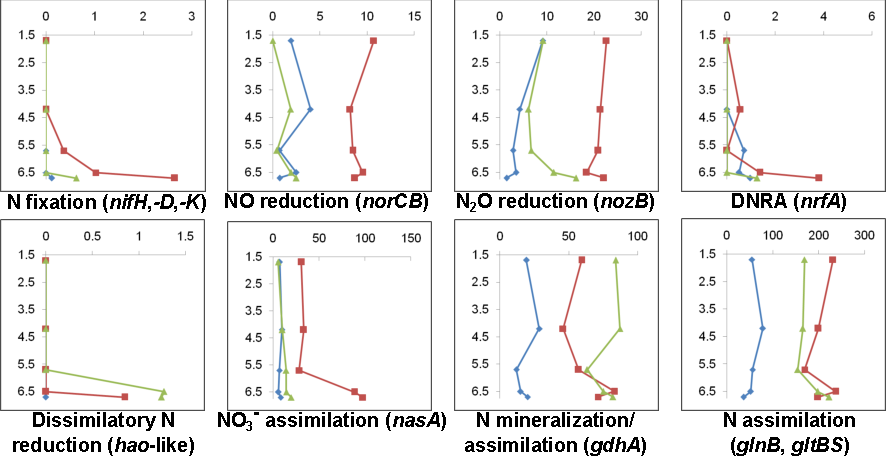
\includegraphics{orglake_figures/n_cycle.pdf}
\caption[Vertical profiles of potential for nitrogen cycling in Organic Lake]{Vertical profiles of potential for nitrogen conversions for each size fraction in Organic Lake. The y-axis shows sample depths (m) and the x-axis shows counts of marker genes normalised to 100 Mbp of \textsc{DNA} sequence. The 0.1, 0.8, 3.0 \textmu{}m size fractions are shown as blue, red and green, respectively. Counts for marker genes for the same pathway or enzyme complex were averaged and those from different pathways were summed. For marker gene descriptions see \tabref{tab:KO_table} and \tabref{tab:marker_genes}.}
\label{fig:n_cycle}

\end{figure}
 
Glutamate dehydrogenase (GDH) genes (\emph{gdhA}) were abundant \figref{fig:n_cycle}, and linked predominantly to \emph{Alpha}- and \emph{Gammaproteobacteria} and to a lesser extent \emph{Bacteroidetes} \tabref{n_cycle_sp}. 
However, the functional significance of the readily reversible GDH depends on its origin; \emph{Bacteroidetes} are likely to use GDH in the oxidative direction for glutamate catabolism \cite{Williams2012}, whereas the use of GDH in the oxidative or reductive directions by \emph{Proteobacteria} is likely to depend upon the source of reduced nitrogen (ammonia vs amino acids). 
Glutamine synthetase (\emph{glnB}) and glutamate synthase genes (\emph{gltBS}), were predominantly linked to \emph{Alpha}- and\emph{Gammaproteobacteria} \tabref{n_cycle_sp}, indicating the potential for high-affinity ammonia assimilation by these groups in Organic Lake. 
The high ammonia concentration in the deep zone (\figreft{fig:vert_struc}, \tabreft{tab:physico-chem}) would result from a higher rate of mineralisation (ammonification) than assimilation. 
This is consistent with abundant \acp{OTU} for \emph{Psychroflexus}(\emph{Bacteroidetes}) in this zone, and due to either turnover of organic matter or lysis of \emph{Bacteroidetes} cells after sedimentation in anoxic water. 
In addition, the gene for ammonia-generating nitrite reductase (\emph{nrfA}) was linked to \emph{Bacteroidetes} and \emph{Planctomycetes} \tabref{tab:n_cycle_sp}, indicating ammonia may also be produced by these putative aerobic heterotrophs. 
Overall, the data suggest that ammonia is actively assimilated in the aerobic upper mixed zone, but is permitted to accumulate in the anaerobic deep zone.
\begin{table}
\footnotesize
\caption[Taxonomic origin of genes involved in nitrogen conversions]{Contribution of different taxonomic groups to counts of marker genes involved in nitrogen conversions.
The taxon with the largest contribution to each process is highlighted in blue. 
}
\label{tab:n_cycle_sp}
\smallskip
\begin{tabularx}{\textwidth}{p{3.5cm}p{0.6cm}p{0.8cm}p{0.8cm}p{0.6cm}p{0.5cm}p{1cm}XX}
\toprule
\textbf{Taxon} & \rotatebox{45}{\textbf{N fixation}} & \rotatebox{45}{\textbf{NO reduction}} & \rotatebox{45}{\textbf{N$_2$O reduction}} & \rotatebox{45}{\textbf{DNRA}} & \rotatebox{45}{\textbf{\emph{hao}}} & \rotatebox{45}{\textbf{N mineralisation}} & \rotatebox{45}{\textbf{NO$_3^-$ assimilation}} & \rotatebox{45}{\textbf{N assimilation}} \\
\midrule
\textbf{\emph{Acidobacteria}} & 0 & 0 & 0 & 0 & 0 & 0.07 & 0 & 0.08 \\
\textbf{\emph{Actinobacteria}} & 0 & 0 & 0 & 0.03 & 0 & 0.32 & 0 & 5.41 \\
\textbf{\emph{Alphaproteobacteria}} & 0.01 & 0.12 & 0 & 0 & 0 & \cellcolor{blue!25}6.39 & 5.49 & 49.4 \\
\textbf{\emph{Aquificae}} & 0 & 0 & 0.26 & 0 & 0 & 0 & 0 & 0.06 \\
\textbf{\emph{Bacteroidetes}} & 0 & 0 & 3.00 & \cellcolor{blue!25}0.27 & 0 & 3.90 & 0.03 & 15.5 \\
\textbf{\emph{Betaproteobacteria}} & 0 & 0.03 & 0 & 0 & 0 & 0.06 & 0.41 & 19.2 \\
\textbf{\emph{Chlorobi}} & 0.03 & 0 & 0 & 0 & 0 & 0.2 & 0 & 0.31 \\
\textbf{\emph{Chloroflexi}} & 0 & 0 & 0 & 0 & 0 & 0.03 & 0 & 0.03 \\
\textbf{\emph{Chrysiogenetes}} & 0 & 0 & 0 & 0 & 0 & 0.01  & 0 & 0.06 \\
\textbf{\emph{Cyanobacteria}} & 0 & 0 & 0 & 0 & 0 & 0.29 & 0 & 0.10 \\
\textbf{\emph{Deferribacteres}} & 0 & 0 & 0 & 0 & 0 & 0 & 0 & 0 \\
\textbf{\emph{Deinococcus-Thermus}} & 0 & 0 & 0 & 0 & 0 & 0.01 & 0 & 0.11 \\
\textbf{\emph{Deltaproteobacteria}} & 0.04 & 0.01 & 0 & 0.07 & \cellcolor{blue!25}0.22 & 0.23 & 0 & 0.58 \\
\textbf{\emph{Epsilonproteobacteria}} & \cellcolor{blue!25}0.32 & 0 & 0 & 0 & 0 & 0.05 & 0 & 1.49 \\
\textbf{\emph{Firmicutes}} & 0.03 & 0 & 0 & 0.03 & 0 & 0.70 & 0 & 3.16 \\
\textbf{\emph{Fornicata}} & 0 & 0 & 0 & 0 & 0 & 0.02 & 0 & 0 \\
\textbf{\emph{Fusobacteria}} & 0 & 0 & 0 & 0 & 0 & 0 & 0 & 0.04 \\
\textbf{\emph{Gammaproteobacteria}} & 0 & \cellcolor{blue!25}3.91 & \cellcolor{blue!25}8.28 & 0 & 0 & 4.75 & \cellcolor{blue!25}14.1 & \cellcolor{blue!25}50.6 \\
\textbf{\emph{Nitrospirae}} & 0 & 0 & 0 & 0.03 & 0 & 0.01 & 0 & 0 \\
\textbf{\emph{Planctomycetes}} & 0 & 0.01 & 0 & 0.16 & 0 & 0 & 0 & 0.26 \\
\textbf{\emph{Spirochaetes}} & 0 & 0.01 & 0 & 0 & 0 & 0.11 & 0 & 0.15 \\
\textbf{\emph{Thermobaculum}} & 0 & 0 & 0 & 0 & 0 & 0.10 & 0 & 0 \\
\textbf{\emph{Thermotogae}} & 0 & 0 & 0 & 0 & 0 & 0 & 0 & 0 \\
\textbf{\emph{Verrucomicrobia}} & 0 & 0 & 0.17 & 0.03 & 0 & 0.25 & 0 & 0.82 \\
 &  &  &  &  &  &  &  &  \\
\textbf{\emph{Crenarchaeota}} & 0 & 0 & 0 & 0 & 0 & 0.02 & 0 & 0 \\
\textbf{\emph{Euryarchaeota}} & 0 & 0 & 0 & 0 & 0 & 0.12 & 0.09 & 0.10 \\
 &  &  &  &  &  &  &  &  \\
\textbf{\emph{Alveolata}} & 0 & 0 & 0 & 0 & 0 & 0.18 & 0 & 0.03 \\
\textbf{\emph{Euglenozoa}} & 0 & 0 & 0 & 0 & 0 & 0 & 0 & 0 \\
\textbf{\emph{Opistokonta}} & 0 & 0 & 0 & 0 & 0 & 0.15 & 0 & 0.13 \\
\textbf{\emph{Rhodophyta}} & 0 & 0 & 0 & 0 & 0 & 0 & 0 & 0.02 \\
\textbf{\emph{Strameopiles}} & 0 & 0 & 0 & 0 & 0 & 0.03 & 0 & 0.15 \\
\textbf{\emph{Viridiplantae}} & 0 & 0 & 0 & 0 & 0 & 0.03 & 0 & 0.35 \\
\bottomrule
\end{tabularx}
\end{table}



Potential for nitrogen conversions typically found in other aquatic environments was greatly reduced in Organic Lake. 
There was a very low potential for nitrogen fixation that was confined to the deep zone \figref{fig:n_cycle} and principally linked to anaerobic \emph{Epsilonproteobacteria} \tabref{tab:n_cycle_sp}. 
This diazotrophic potential may not be realized by \emph{Epsilonproteobacteria}, given the high ammonia concentration present in the deep zone. 
No ammonia monooxygenase genes (\emph{amoA}) were detected.The potential for ammonia oxidation was only represented by hydroxylamine/hydrazine oxidase-like (\emph{hao}) genes, which werein low abundance and linked to \emph{Deltaproteobacteria} \tabref{tab:n_cycle_sp}. 
\emph{hao} genes are present in non-ammonia-oxidising bacteria \cite{Bergmann2005}, and those from Organic Lake belong to a family of multiheme cytochrome c genes present in sulphate-reducing \emph{Deltaproteobacteria} that have no proven role in ammonia oxidation. 
In the genomes of sulphate-reducing \emph{Deltaproteobacteria} thehao gene is invariably situated adjacent to a gene for a NapC/NirT protein, which suggests a role in dissimilatory nitrate reduction. 
Collectively these data indicate an inability for nitrification to occur in the upper mixed zone and no potential for ammonia loss in the deep zone.

Denitrification genes (\emph{norCB} and \emph{nozB}) and genes for nitrate assimilation (\emph{nasA}) were present throughout the water column \figref{fig:n_cycle} and were linked primarily to \emph{Gammaproteobacteria} \tabref{tab:n_cycle_sp}. 
Low nitrate and nitrite in the deep zone (\figreft{fig:vert_struc}, \tabreft{tab:physico-chem}) indicates oxidized nitrogen has been depleted by dissimilatory or assimilitory reduction by heterotrophic \emph{Gammaproteobacteria}. 
Denitrification genes are phylogenetically widespread and usually induced by low oxygen or oxidized nitrogen species \cite{Kraft2011} and thus expected to be active in the deep zone or oxycline. 
However, denitrification may be inhibited even if conditions appear appropriate. 
For example, in Lake Bonney, Antarctica, denitrification occurs in the west lobe, but not in the east lobe of the lake despite the presence of anoxia, nitrate and denitrifying \emph{Marinobacter} species \cite{Ward1997, Ward2005}.
 Moreover, in the absence of nitrification, denitrification and nitrate assimilation would be limited by the lack of potential to re-form oxidized nitrogen. 
The preponderance of assimilation/mineralisation pathways geared towards reduced nitrogen appears to reflect a ``short circuit'' of the typical nitrogen cycle that would conserve nitrogen in a largely closed system. 
Hence, the predominant nitrogen source is regenerated fixed nitrogen.
Similar findings were also made for Ace Lake, although in this system the presence of a dense layer of green sulphur bacteria with the potential to fix nitrogen augments the nitrogen cycle \cite{Lauro2011}. 

\subsection{Molecular basis for unusual sulphur chemistry}
Several meromictic hypersaline lakes in the Vestfold Hills,including Organic Lake, with practical salinity $>$150 are characterized by an absence of hydrogen sulphide and photoautotrophic sulphur bacteria \cite{Burke1988}. 
Although sulphate is present \cite{Franzmann1987b}, geochemical conditions of these lakes are not conducive to dissimilatory sulphur cycling between sulphur oxidising and sulphate reducing bacteria typical of other stratified systems such as Ace Lake \cite{Ng2010a, Lauro2011}. 
Consistent with this, potential for dissimilatory sulphate reduction represented by dissimilatory sulfite reductase (\emph{dsrAB}) and adenylylsulphate reductase (\emph{aprAB})linked to sulphate-reducing \emph{Deltaproteobacteria} \tabref{tab:s_cycle_sp} was low in Organic Lake. 
Sulphate-reduction potential was confined to the 6.7 m sample \figref{fig:s_cycle} where oxygen concentration was lowest and \emph{Deltaproteobacteria} were present \figref{fig:genus_barplots_bact}.
\begin{figure}
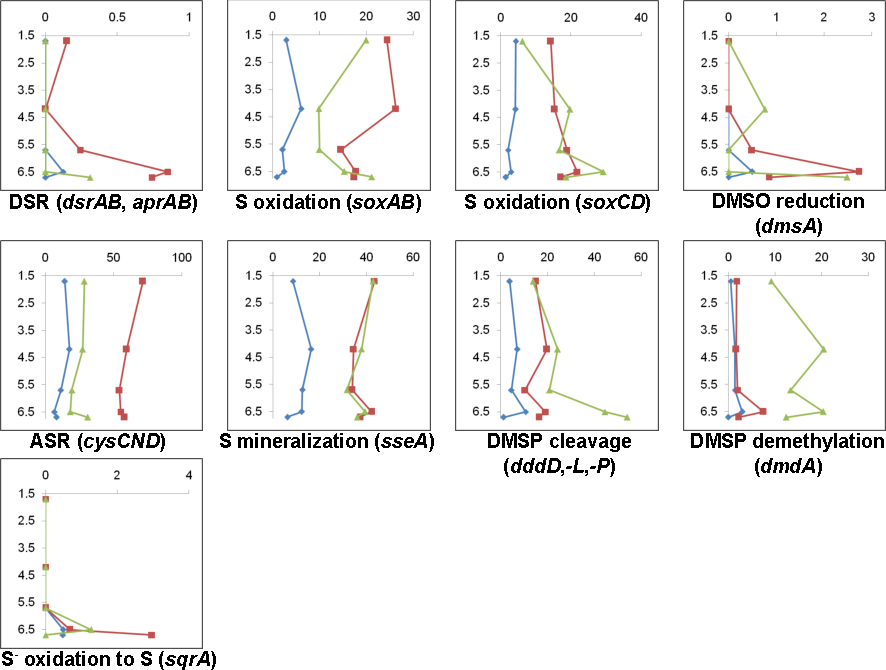
\includegraphics{orglake_figures/s_cycle.pdf}
\caption[Vertical profiles of potential for sulphur cycling in Organic Lake]{Vertical profiles of potential for sulphur conversions for each size fraction in Organic Lake. The y-axis shows sample depths (m) and the x-axis shows counts of marker genes normalised to 100 Mbp of \textsc{DNA} sequence. The 0.1, 0.8, 3.0 \textmu{}m size fractions are shown as blue, red and green, respectively. Counts for marker genes for the same pathway or enzyme complex were averaged and those from different pathways were summed. For marker gene descriptions see \tabref{tab:KO_table} and \tabref{tab:marker_genes}.}
\label{fig:s_cycle}

\end{figure}
 

Capacity for oxidation of reduced sulphur compounds, represented by the sulphur oxidation multienzyme genes (\emph{soxAB}), was present throughout the water column \figref{fig:s_cycle} and linked primarily to \emph{Alpha}- and\emph{Gammaproteobacteria} \tabref{tab:s_cycle_sp}. 
Sulphur-oxidising \emph{Alpha}- and \emph{Gammaproteobacteria} are known to oxidise sulphur compounds, such as thiosulphate, aerobically. 
Although a small proportion of \emph{Gammaproteobacteria} had the capacity for autotrophy 
(see \ref{subs:carbon}), 
the majority of sulphur-oxidizers were likely chemolithoheterotrophs as they were related to heterotrophic \emph{Marinobacter} and \emph{Roseobacter} clade. 
The sulphur dehydrogenase genes \emph{soxCD} linked to \emph{Alpha}- and \emph{Gammaproteobacteria} were similarly present throughout the water column. 
\emph{soxCD} are accessory components of the Sox enzyme system without which complete oxidation of thiosulphate cannot occur \cite{Friedrich2005}. 
Thus the presence of \emph{soxCD} indicates complete oxidisation likely occurs, although the different distribution of \emph{soxAB} and \emph{soxCD} in the water column \figref{fig:s_cycle} suggests a proportion of the community may lack \emph{soxCD} and deposit sulphur. 
\begin{table}
\footnotesize
\caption[Taxonomic origin of genes involved in sulphur conversions]{Contribution of different taxonomic groups to counts of marker genes involved in sulphur conversions.}
\label{tab:s_cycle_sp}
\smallskip
\begin{tabularx}{\textwidth}{p{3.5cm}p{0.8cm}p{0.8cm}p{0.8cm}XXX}
\toprule
\textbf{Taxon} & \rotatebox{45}{ \textbf{DSR} } & \rotatebox{45}{ \textbf{S oxidation} } & \rotatebox{45}{ \textbf{\emph{sqrA} } } & \rotatebox{45}{ \textbf{S assimilation} } & \rotatebox{45}{ \textbf{S mineralisation} } & \rotatebox{45}{ \textbf{DMSO reduction} } \\
\midrule
\textbf{\emph{Acidobacteria}} & 0 & 0 & 0 & 0.03 & 1.03 & 0 \\
\textbf{\emph{Actinobacteria}} & 0 & 0 & 0 & 0.15 & 0 & 0 \\
\textbf{\emph{Alphaproteobacteria}} & 0 & 2.05 & 0 & 0.85 & 11.7 & 0 \\
\textbf{\emph{Aquificae}} & 0 & 0 & 0 & 0 & 0 & 0 \\
\textbf{\emph{Bacteroidetes}} & 0 & 0 & 0 & 5.06 & 0.20 & 0 \\
\textbf{\emph{Betaproteobacteria}} & 0 & 1.09 & 0 & 2.07 & 0.69 & 0 \\
\textbf{\emph{Chlorobi}} & 0 & 0 & 0 & 0.03 & 0.15 & 0 \\
\textbf{\emph{Chloroflexi}} & 0 & 0 & 0 & 0 & 0.30 & 0 \\
\textbf{\emph{Chrysiogenetes}} & 0 & 0 & 0 & 0.01 & 0 & 0 \\
\textbf{\emph{Cyanobacteria}} & 0 & 0 & 0 & 0.13 & 0.05 & 0 \\
\textbf{\emph{Deferribacteres}} & 0 & 0 & 0 & 0 & 0 & 0 \\
\textbf{\emph{Deinococcus-Thermus}} & 0 & 0 & 0 & 0 & 0.09 & 0 \\
\textbf{\emph{Deltaproteobacteria}} & \textbf{0.19} & 0 & 0 & 0.56 & 0.20 & 0.03 \\
\textbf{\emph{Epsilonproteobacteria}} & 0 & 0.03 & \textbf{0.39} & 0.13 & 0 & 0 \\
\textbf{\emph{Firmicutes}} & 0 & 0 & 0 & 0.22 & 0.09 & \textbf{0.36} \\
\textbf{\emph{Fornicata}} & 0 & 0 & 0 & 0 & 0 & 0 \\
\textbf{\emph{Fusobacteria}} & 0 & 0 & 0 & 0.03 & 0.13 & 0 \\
\textbf{\emph{Gammaproteobacteria}} & 0 & \textbf{2.64} & 0 & \textbf{22.4} & \textbf{14.0} & 0 \\
\textbf{\emph{Nitrospirae}} & 0 & 0 & 0 & 0 & 0 & 0 \\
\textbf{\emph{Planctomycetes}} & 0 & 0 & 0 & 0.03 & 0 & 0 \\
\textbf{\emph{Spirochaetes}} & 0 & 0 & 0 & 0 & 0.03 & 0.12 \\
\textbf{\emph{Thermobaculum}} & 0 & 0 & 0 & 0 & 0.08 & 0 \\
\textbf{\emph{Thermotogae}} & 0 & 0 & 0 & 0.01 & 0 & 0 \\
\textbf{\emph{Verrucomicrobia}} & 0 & 0 & 0 & 0.18 & 0 & 0 \\
 &  &  &  &  &  &  \\
\textbf{\emph{Crenarchaeota}} & 0.02 & 0 & 0 & 0 & 0 & 0 \\
\textbf{\emph{Euryarchaeota}} & 0 & 0 & 0 & 0.02 & 0.12 & 0 \\
 &  &  &  &  &  &  \\
\textbf{\emph{Alveolata}} & 0 & 0 & 0 & 0 & 0 & 0 \\
\textbf{\emph{Euglenozoa}} & 0 & 0 & 0 & 0 & 0.03 & 0 \\
\textbf{\emph{Opistokonta}} & 0 & 0 & 0 & 0.11 & 0.03 & 0 \\
\textbf{\emph{Rhodophyta}} & 0 & 0 & 0 & 0 & 0 & 0 \\
\textbf{\emph{Strameopiles}} & 0 & 0 & 0 & 0 & 0 & 0 \\
\textbf{\emph{Viridiplantae}} & 0 & 0 & 0 & 0.03 & 0.15 & 0 \\
\bottomrule
\end{tabularx}
\end{table}



Sulphur-oxidising \emph{Epsilonproteobacteria} possessing \emph{soxAB} genes \tabref{tab:s_cycle_sp} were present only in the deep zone of Organic Lake \figref{fig:genus_barplots_bact} and were related to autotrophic deep sea sulphur-oxidisers, some members of which are capable of anaerobic sulphur oxidation using nitrate \cite{Yamamoto2011}. 
It is unlikely that appreciable sulphur oxidation occurs in the deep zone as the known terminal electron acceptors, oxygen and nitrate, are deplete and the abundance of sulphur oxidising \emph{Epsilonproteobacteria} is low \figref{fig:genus_barplots_bact}. 
\emph{Epsilonproteobacteria} were also linked to a capacity for oxidation of sulphide to elemental sulphur by utilising sulphide:quinone oxidoreductase (\emph{sqrA}) (\figreft{fig:s_cycle}, \tabreft{tab:s_cycle_sp}). 
In this pathway, sulphur is released as polysulphides, which is a potential biological source of the abundant polysulphides that have been detected in the lake \cite{Roberts1993b}.

It is likely that the limited anaerobic dissimilatory sulphur cycle contributes to the accumulation of \ac{DMS} in Organic Lake in the deep zone.
In the upper mixed zone, \ac{DMS} could potentially be oxidized as a carbon and energy source or utilized as an electron donor by sulphur-oxidising bacteria \cite{Schafer2010}. 
In anoxic zones, methanogenic \emph{Archaea} or sulphate-reducing bacteria are the main organisms known to breakdown \ac{DMS} \cite{Schafer2010}. 
Methanogens and genes involved in methanogenesis were not detected, nor has methane been detected \cite{Gibson1994} leaving sulphate-reduction the most likely route of \ac{DMS} catabolism. 
The low dissimilatory sulphate reduction potential in the deep zone coupled with the relatively stagnant waters would likely minimize \ac{DMS} oxidation and loss by ventilation. \ac{DMS} would therefore be expected to accumulate in the deep zone if production rates were higher than breakdown.

To determine the source of high \ac{DMS} in the bottom waters of Organic Lake, the genes involved in \ac{DMS} formation were surveyed.
 Genes for \ac{DMSP} lyases \emph{dddD}, \emph{dddL} and \emph{dddP}, were detected in Organic Lake at levels comparable to other dominant processes such as respiration and fermentation \figref{fig:s_cycle} indicating \ac{DMSP} is an important carbon and energy source in Organic Lake. 
\emph{dddD} was the most abundant of the Organic Lake \ac{DMSP} lyases \tabref{tab:metag_compare} and comprised two main types: MAR-dddD and OL-dddD \figref{fig:dddD_tree}.
\begin{figure}
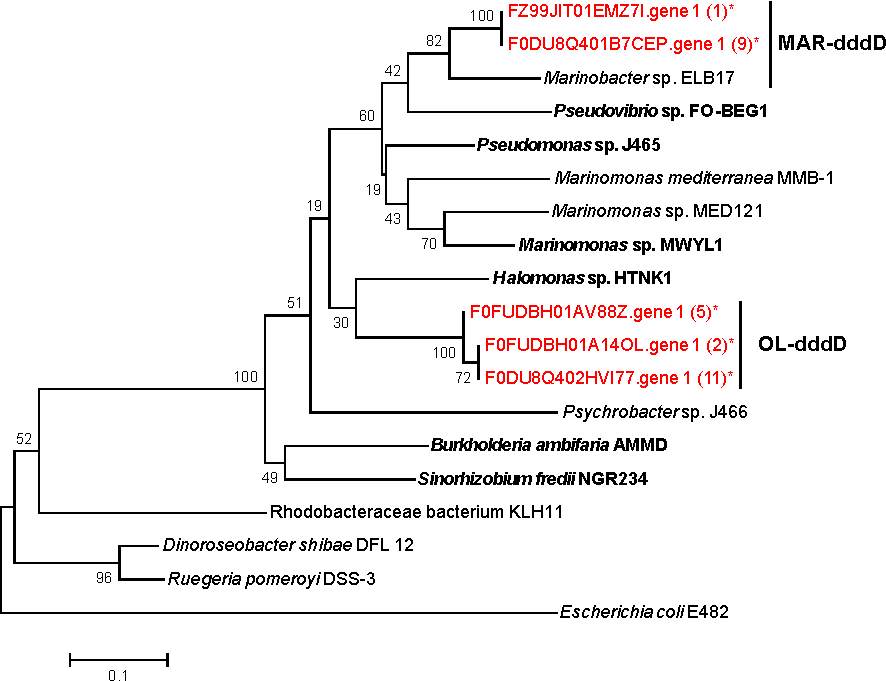
\includegraphics[width=\textwidth]{orglake_figures/dddD_tree.pdf}
\caption[Phylogenetic tree of DddD DMSP lyase homologues]{Phylogenetic tree of DddD DMSP lyase homologues. \emph{E. coli} carnitine coenzyme A transferase was used as an outgroup. \emph{Dinoroseobacter shibae} DFL 12 and \emph{Ruegeria pomeroyi} DSS-3 homologues are a non-functional outgroup \cite{Todd2011}. The tree was computed from a 75 amino acid region within the conserved amino-terminal class III coenzyme A domain (CaiB) using the neighbour-joining algorithm. Organic Lake sequences from this study are shown in red and marked with an asterisk (*). Numbers in parentheses are counts of sequences that clustered with the Organic Lake homologue shown in the tree with 90\% amino acid identity. Sequences with confirmed DMSP lyase activity are shown in bold. Accession numbers from top to bottom are: EBA01716, AEV37420, ACY01992, ADZ91595, EAQ63474, ABR72937, ACV84065, ACY02894, ABI89851, YP\_002822700, EEE36156, ABV95365, AAV94987 and EGB36199.}
\label{fig:dddD_tree}

\end{figure}
 
Neither of these types clustered with the non-functional \emph{Dinoroseobacter shibae} DFL 12 and \emph{Ruegeria pomeroyi} DSS-3 \emph{dddD} homologues \cite{Todd2011} or carnitine coenzyme A transferase outgroups, thereby providing support for their proposed role as functional \ac{DMSP} lyases. 
The MAR-dddD type includes the \emph{Marinobacter} sp. ELB17 \emph{dddD} homologue, and MAR-dddD sequences were most abundant on the 0.8 \textmu{}m fraction where \emph{Marinobacter} \acp{OTU} were also abundant, indicating MAR-dddD derives from Organic Lake \emph{Marinobacter} \figref{fig:dddD_tree}. 
OLn-dddD did not have a close relative from cultured bacteria making its precise taxonomic origins uncertain. 
The abundance of OL-dddD on the 3.0 \textmu{}m fraction suggests it originates from \emph{Alphaproteobacteria}. 
OL-dddD containing contigs carried genes of mixed \emph{Alpha}- and \emph{Gammaproteobacteria}l origin supporting its provenance from one of these classes and consistent with the ``pick n' mix'' arrangement of genes found beside sequenced \emph{dddD} regions \cite{Johnston2008} \figref{fig:OLdddD_scaffolds}. 
Adjacent to OL-dddD was \emph{dddT} \figref{fig:OLdddD_scaffolds}, a betaine, choline, carnitine transporter (BCCT) family protein that likely functions in substrate import, demonstrating OL-dddD forms an operon-like structure,similar to \emph{Halomonas} sp. HTNK1 \cite{Todd2010}.
\begin{figure}
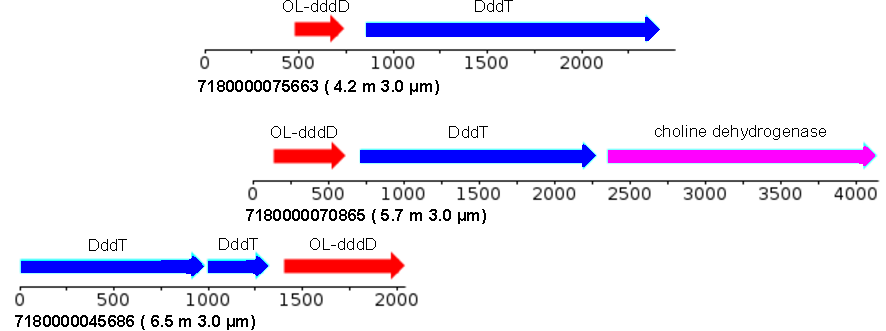
\includegraphics[width=\textwidth]{orglake_figures/OLdddD_scaffolds.pdf}
\caption[Genomic maps of Organic Lake scaffolds containing the OL-dddD homologue]{Genomic maps of Organic Lake scaffolds containing the OL-dddD homologue. DddT and choline dehydrogenase had best \ac{BLAST} matches to \emph{Halomonas} sp. HTNK1 (\emph{Gammaproteobacteria}) and \emph{Hoeflea phototrophica} DFL-43 (\emph{Alphaproteobacteria}), respectively. The numbers represent base pairs. The sample depth and filter from which the scaffold was assembled is shown in parentheses beside the scaffold ID.}
\label{fig:OLdddD_scaffolds}

\end{figure}


Two \emph{dddL} groups were detected in Organic Lake: SUL-dddL and MAR-dddL \figref{fig:dddL_tree}. 
\begin{figure}
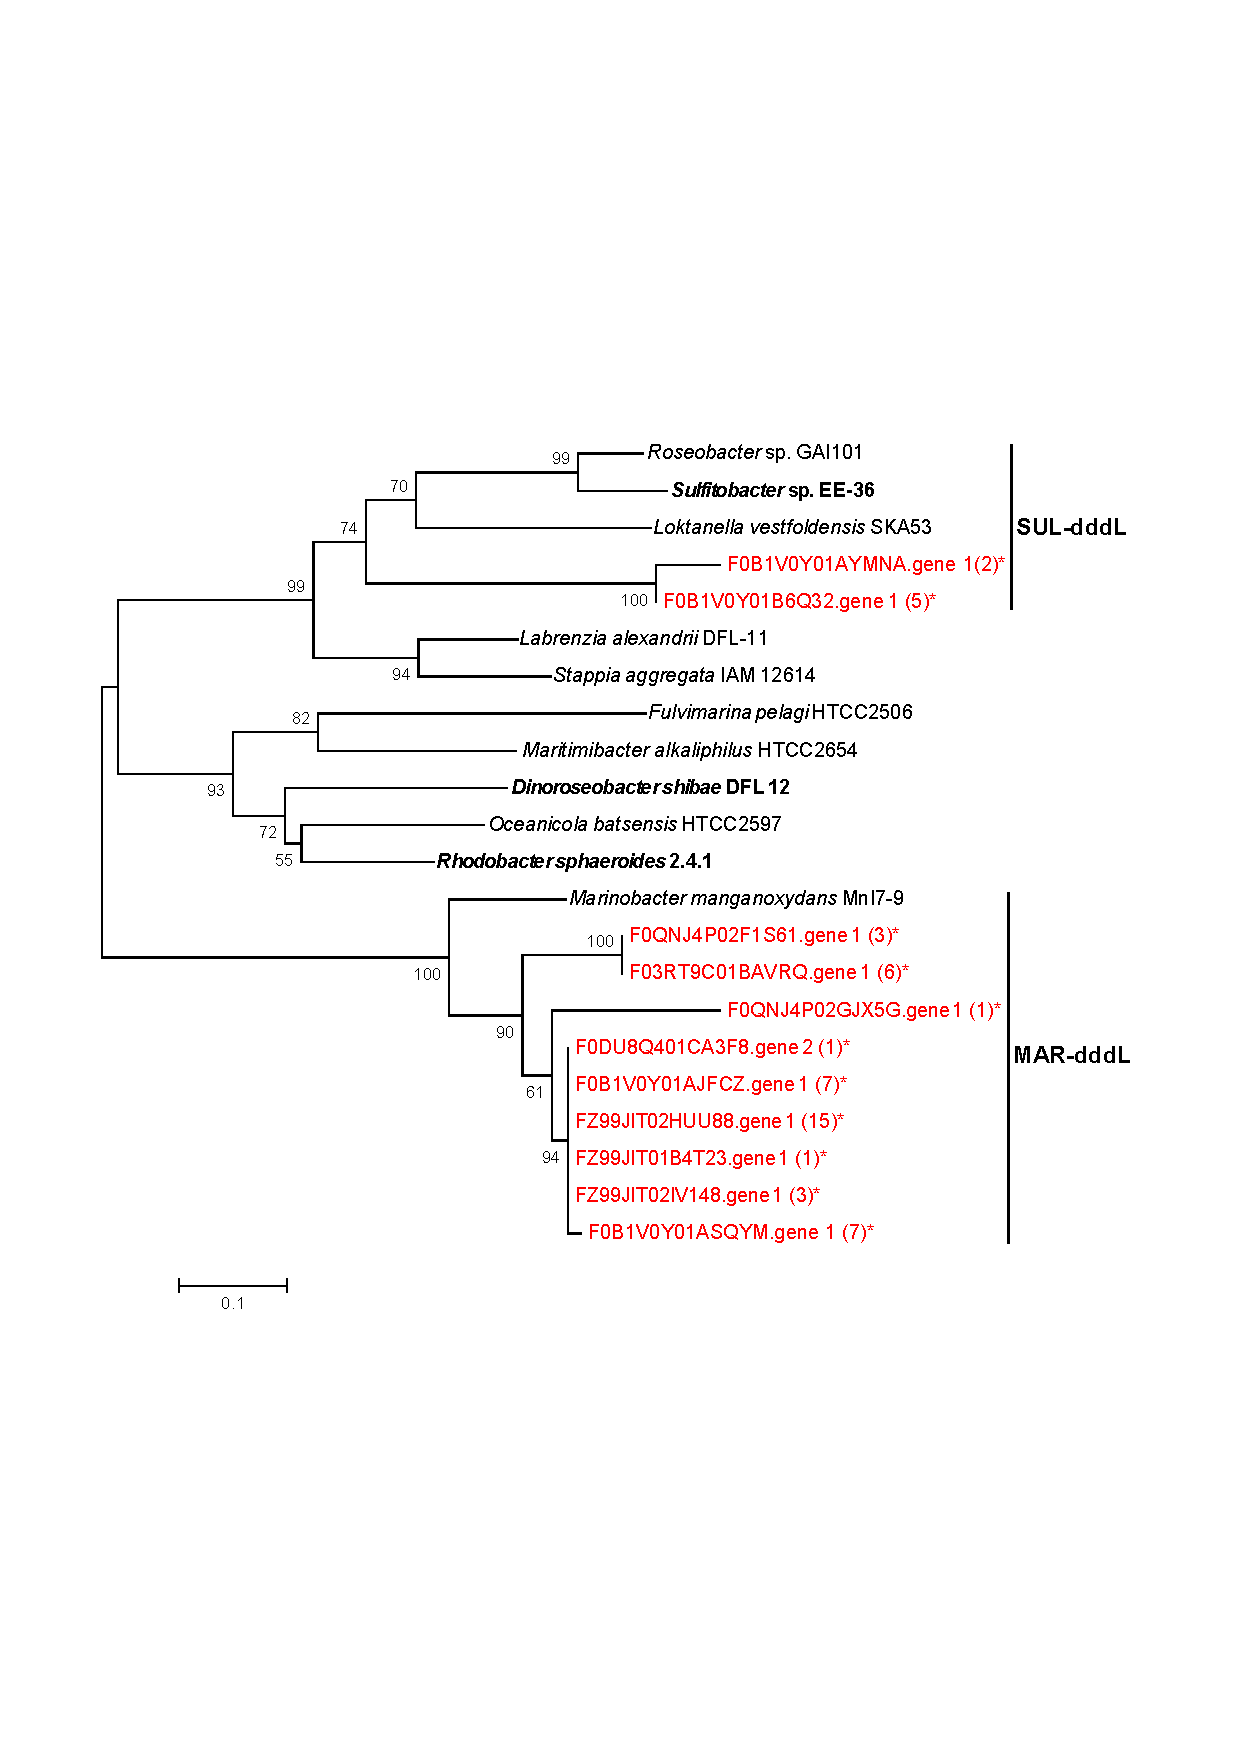
\includegraphics[width=\textwidth]{orglake_figures/dddL_tree.pdf}
\caption[Phylogeny of DddL DMSP lyase homologues]{Phylogeny of DddL DMSP lyase homologues. The tree was computed from an 84 amino acid N-terminal region using the neighbour-joining algorithm. Organic Lake sequences from this study are shown in red and marked with an asterisk (*). Numbers in parentheses are counts of sequences that clustered with the Organic Lake homologue shown in the tree with 90\% amino acid identity. Sequences with confirmed DMSP lyase activity are shown in bold. Accession numbers from top to bottom are: EEB86351, ADK55772, EAQ07081, EEE47811, EAV43167, EAU41122, EAQ10619, ABV95046, EAQ04071, ABA77574 and EHJ04839.}
\label{fig:dddL_tree}

\end{figure}

The former includes the \emph{Sulfitobacter} sp. EE-36 \emph{dddL} and the latter the \emph{Marinobacter manganoxydans} MnI7-9 homologue indicating they originate from \emph{Roseobacter} clade and \emph{Gammaproteobacteria}, respectively. 
\emph{Sulfitobacter} sp. EE-36 has demonstrated \ac{DMSP} lyase activity and the \emph{dddL} gene alone is sufficient for \ac{DMS} generation \cite{Curson2008}. 
These data indicate that the Organic Lake members of the SUL-dddL group perform the same functional role. 
The MAR-dddL clade appears to be an uncharacterized branch of the \emph{dddL} family. 
emph{dddP} was detected as the least abundant of the \ac{DMSP} lyases \tabref{tab:metag_compare}. 
Phylogenetic analyses showed Organic Lake \emph{dddP} likely originate from \emph{Roseovarius} \figref{fig:dddP_tree}. 
The Organic Lake sequences formed a clade with the functionally verified \emph{Roseovarius nibinhibens} ISM \emph{dddP} \cite{Todd2009}. 
\begin{figure}
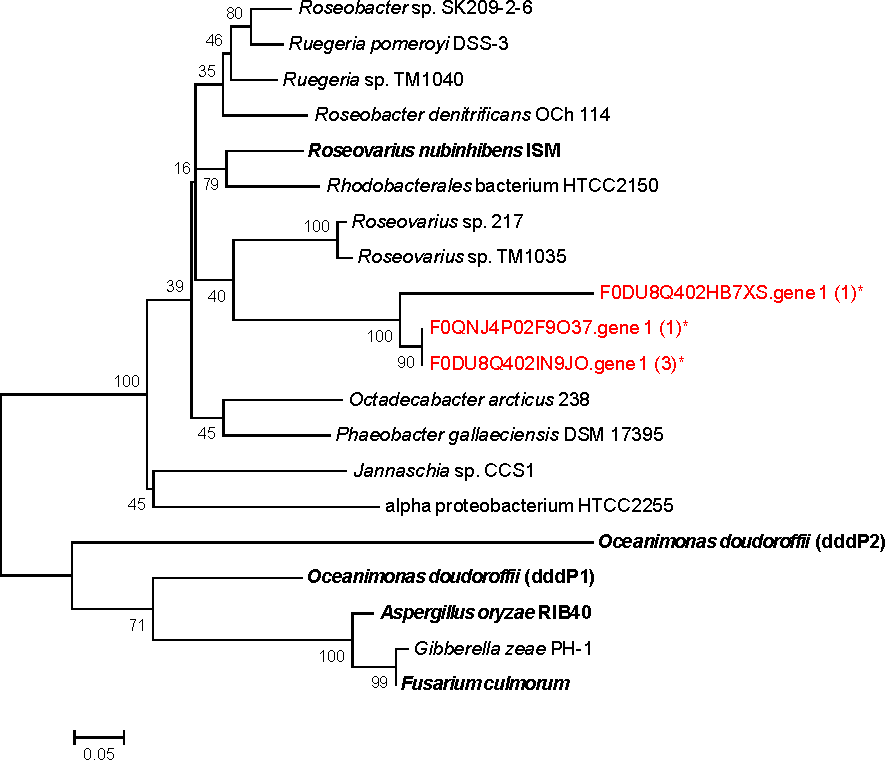
\includegraphics[width=\textwidth]{orglake_figures/dddP_tree.pdf}
\caption[Phylogenetic tree of DddP DMSP lyase homologues]{Phylogenetic tree of DddP DMSP demethylase homologues. The tree was computed from a 129 amino acid C-terminal region using the neighbour-joining algorithm. Organic Lake sequences from this study are shown in red and marked with an asterisk (*). Numbers in parentheses are counts of sequences that clustered with the Organic Lake homologue shown in the tree with 90\% amino acid identity. Sequences with confirmed DMSP lyase activity are shown in bold. Accession numbers from top to bottom are: ZP\_01755203, YP\_167522, YP\_613011, YP\_682809, EAP77700, ZP\_01741265, ZP\_01036399, ZP\_01881042, ZP\_05063825, AFO91571, YP\_509721, ZP\_01448542, AEQ39103, AEQ39091, XP\_001823911, XP\_389272 and ACF19795.}
\label{fig:dddP_tree}

\end{figure}


A single type of \ac{DMSP} demethylase, \emph{dmdA} was identified. 
It clustered with \emph{Roseobacter} clade \emph{dmdA} \figref{fig:dmdA_tree}, corresponding to the marine clade A \cite{Howard2006}, and includes the functionally verified \emph{R. pomeroyi} DSS-3 homologue. 
\begin{figure}
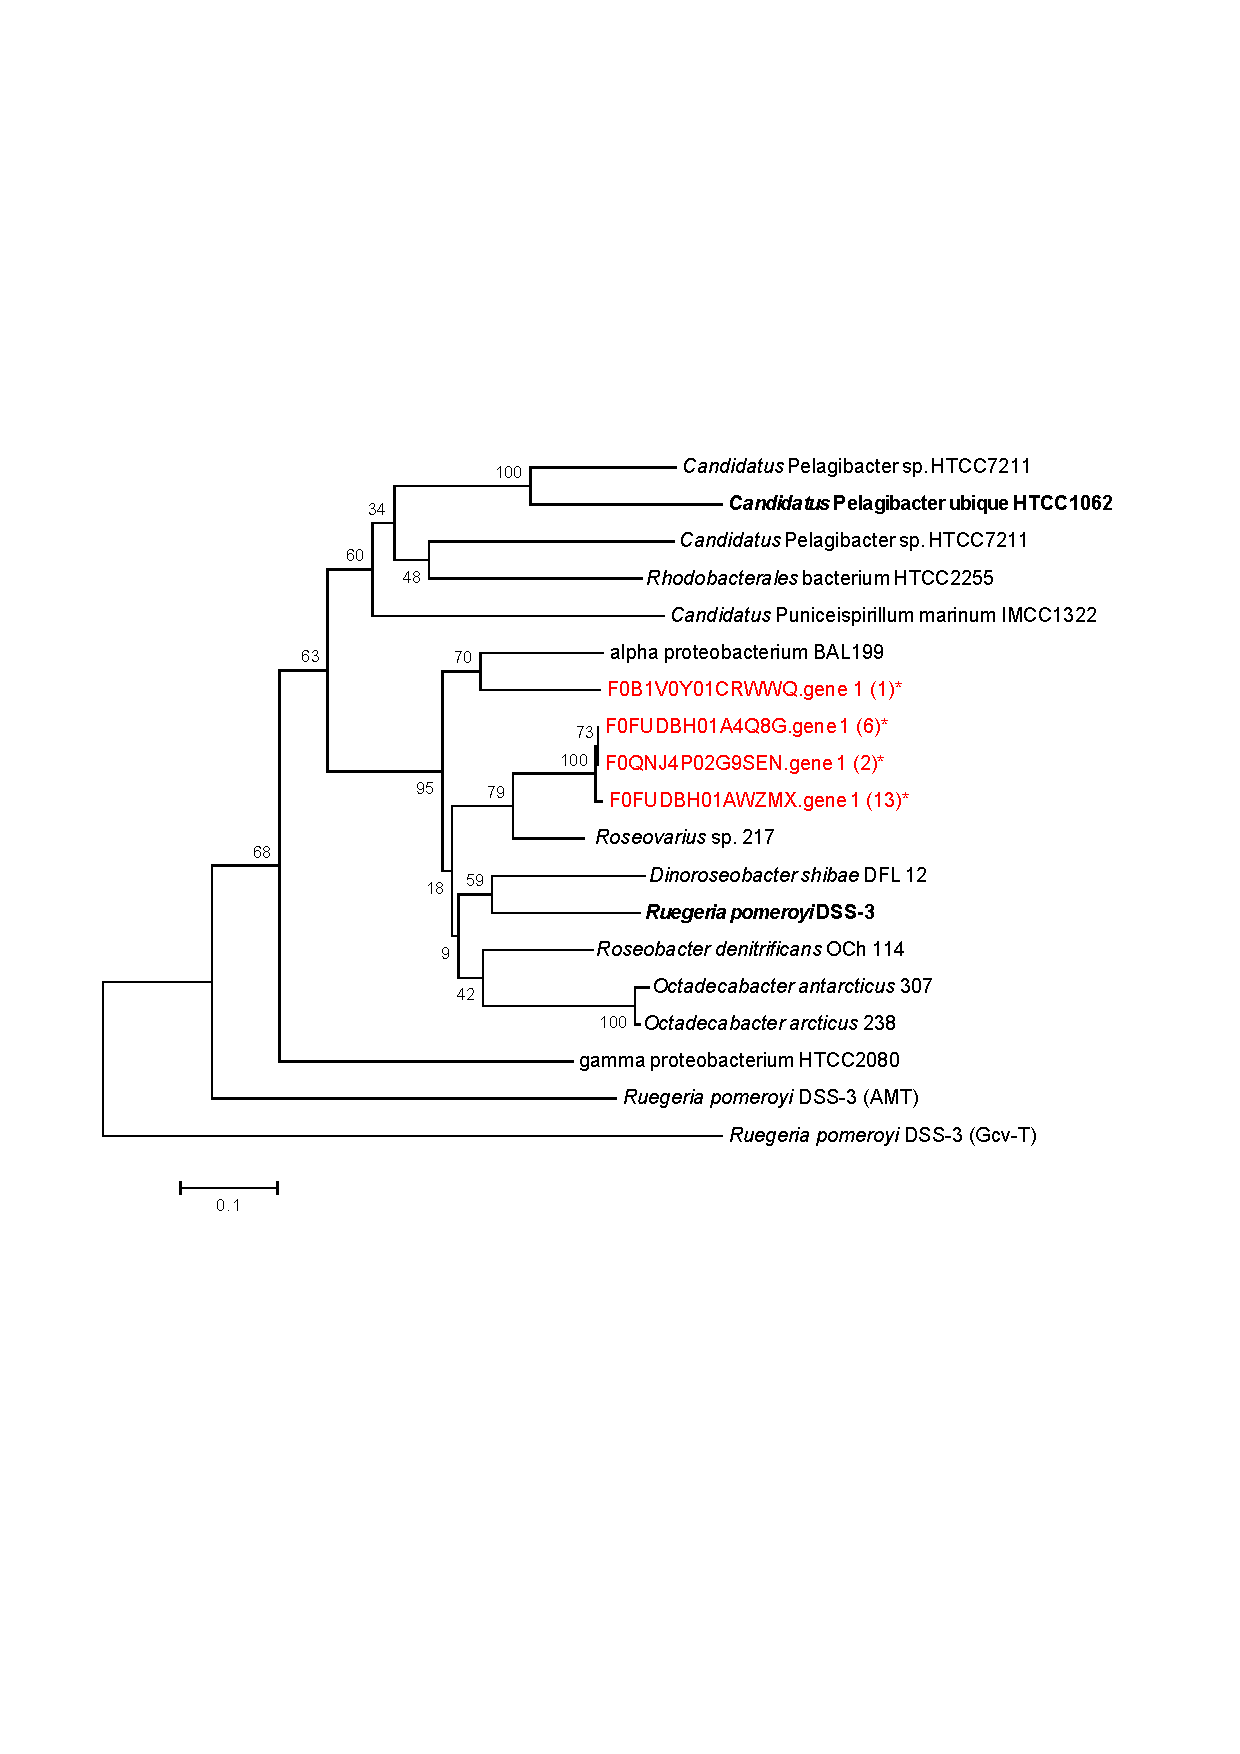
\includegraphics{orglake_figures/dmdA_tree.pdf}
\caption[Phylogenetic tree of DmdA DMSP demethylase homologues]{Phylogenetic tree of DmdA DMSP demethylase homologues. The tree was computed from a 128 amino acid region using the neighbour-joining algorithm. Organic Lake sequences from this study are shown in red and marked with an asterisk (*). Numbers in parentheses are counts of sequences that clustered with the Organic Lake homologue shown in the tree with 90\% amino acid identity. Sequences with confirmed DMSP demethylase activity are shown in bold. Accession numbers from top to bottom are: EDZ60447, YP\_265671, EDZ61098, EAU51039, YP\_003550401, EDP61332, EAQ26389, ABV94056, AAV94935, AAV95190, EDY79173, EDY89914, EAW42451, AAV94935 and AAV97197.}
\label{fig:dmdA_tree}

\end{figure}

These data indicate that the Organic Lake sequences correspond to true \ac{DMSP} demethylases and not related glycine cleavage T proteins or aminomethyltransferases \cite{Howard2006}. 
\ac{DMSP} cleavage appears to be a significant source of \ac{DMS} in Organic Lake. 
\ac{DMSP} likely originates from \emph{Bacillariophyta} or \emph{Dinoflagellida} as Organic Lake \emph{Dunaliella} have been reported not to produce \ac{DMSP} in culture \cite{Franzmann1987b}. 
Based on the abundance of marker genes, \ac{DMSP} cleavage is predicted to occur at highest levels in the deep zone \figref{fig:s_cycle} where the \ac{DMS} concentration has been measured to be highest \cite{Deprez1986, Franzmann1987b, Gibson1991, Roberts1993a, Roberts1993b}. 
\ac{DMS} can also be produced in anoxic environments from the reduction of \ac{DMSO}, degradation of sulphur containing amino acids, and sulphide methylation \cite{Schafer2010}. 
Our data indicate that some \ac{DMSO} reduction linked to \emph{Firmicutes} could occur, but is not likely a major pathway \figref{fig:s_cycle}, and the potential for the other \ac{DMS} yielding processes could not be determined because the enzymes involved in these pathways have not been established. 
When cultivated, Halomonas isolates from Organic Lake produced \ac{DMS} from cysteine \cite{Franzmann1987b} providing some evidence that \ac{DMS} production from anaerobic degradation of amino acids can occur. 
Abiotic pathways for anaerobic production of \ac{DMS} have also been proposed \cite{Roberts1993b}.

The potential for \ac{DMSP} cleavage was more than twice that of \ac{DMSP} demethylation \figref{fig:s_cycle}. 
This is unusual compared to the marine environment or Ace Lake where \ac{DMSP} demethylation potential is much higher than cleavage \tabref{tab:metag_compare}. 
Previous estimates have similarly shown marine environments to have demethylation potential up to two orders of magnitude higher than cleavage \cite{Howard2008, Todd2009, Todd2011, Reisch2011b}. 
The frequency of \ac{DMSP} lyase genes \emph{dddD} and \emph{dddL} in Organic Lake exceeded those of all other environments, except Punta Cormorant hypersaline lagoon, where dddL abundance was comparable \tabref{tab:metag_compare}. 
This suggests selection in Organic Lake for \ac{DMSP} cleavage due to functional advantage and/or selection for taxa that carry \ac{DMSP} lyase genes. 
There is evidence that high \ac{DMSP} cleavage potential is adaptive in hypersaline systems, as a high proportion of ddd genes were similarly detected in Punta Cormorant hypersaline lagoon and saltern ponds \cite{Raina2010}. Determination of the taxonomic composition of these other hypersaline environments could indicate whether selection is occuring for functional capacity or on a taxonomic level if the taxonomic composition between these systems was significantly different but abundance of DMSP lyase genes were high.

The accumulated \ac{DMS} in Organic Lake suggests conditions in Organic Lake favor the relatively inefficient lysis pathway, where both sulphur and carbon is lost to the organism performing the \ac{DMSP} lysis, over the more `thrifty' demethylation pathway. 
This is particularly pertinent to the \emph{Roseobacter} lineages that can also perform either process. 
One possibility that has been proposed is that when sulphur is in excess and the organism can easily assimilate alternative sulphur sources, the lysis pathway may be competitive \cite{Johnston2008}. 
This may be particularly the case in hypersaline systems if higher concentrations of \ac{DMSP} are being produced as an osmolyte.

\section{Conclusions}
Through the use of shotgun metagenomics and size partitioning of samples, we discovered that the Organic Lake system is dominatedby heterotrophic bacteria related to \emph{Psychroflexus}, \emph{Marinobacter} and \emph{Roseovarius} with primary production provided largely by chlorophyte algae related to \emph{Dunaliella}. 
Genetic potential for oxidation of fixed carbon by heterotrophic bacteria occurs greatly in excess of carbon fixation, suggesting possible net carbon loss. 
However, by linking key metabolic processes to the dominant heterotrophic lineages we uncovered processes that were unusually abundant in Organic Lake that may serve to maximize exploitation of limited resources and minimize loss. 
Recalcitrant polymeric algal material and particulate matter is likely remineralized by \emph{Psychroflexus} in the upper mixed zone and by \emph{Firmicutes} in the deep zone to provide labile substrates for use by other heterotrophic bacteria. 
The generalist \emph{Marinobacter} and \emph{Roseovarius} lineages were associated with abundant genes involved in rhodopsin-mediated and \ac{AAnP} photoheterotrophy; the latter of which was more abundant in Organic Lake than any other system surveyed. 
Potential for chemolithoheterotrophy, sulphur oxidation and CO oxidation was also high, and along with photoheterotrophy, may provide a supplementary energy source if organic carbon becomes limiting.

In addition to being able to describe the functional capacities and potential importance of poorly understood microbial processes occurring in the lake (e.g. photoheterotrophy by \emph{Alphaproteobacteria}), we were able to answer targeted questions about the biology of the unusual lake sulphur chemistry. 
The low potential for dissimilatory sulphur cycling in the deep zone and relatively stable waters, combined with the generation of \ac{DMS} from \ac{DMSP}, facilitate the accumulation of a high level of \ac{DMS} in the lake. 
It appears \emph{Marinobacter} and \emph{Roseovarius} play a key role in \ac{DMS} formation by cleaving \ac{DMSP} generated by upper mixed zone eucaryal algae. 
The remarkable abundance of \ac{DMSP} lyase genes suggests \ac{DMSP} is a significant carbon source in Organic Lake and the cleavage pathway provides a selective advantage under the unique constraints of the Organic Lake environment.

In view of the minimal capacity for biological fixation of carbon and nitrogen, and yet organic richness, including high levels of \ac{DMS}, in Organic Lake,we evaluated what input the lake may have received throughout its relatively brief $\sim$3,000 year history. 
The volume of the lake is small ($\sim$6 $\times$ 10$^4$ m$^3$), and exogenous input may occur from guano deposits in a small penguin rookery nearby the lake, through giant petrel or skua predation and defecation, and/or by decaying animal carcasses such as elephant seals which can weigh on the order of 1 ton and are present near the lake. 
It is also possible that during isolation from the ocean, the base of the water column in the marine basin that formed the lake may have acted as a sump for organic material. 
Phytoplankton blooms and benthic mats tend to make coastal marine basins very productive, and organic matter that sediments out of the surface waters will become trapped in the denser, more saline bottom layers \cite{Bird1991}. 
Retention of captured organic matter in the lake may also have been facilitated by Organic Lake having become highly saline quickly \cite{Bird1991}. 
Studies in the future that experimentally determine exogenous input and historical lake dynamics (e.g. stable isotope and biomarker analyses of lake sediment), the role of benthic communities, and metaproteogenomic analyses of interannual community composition and function, will provide improved knowledge of the unusual biogeochemistry of Organic Lake and better enable predictions to be made about how the lake may be affected by ecosystem changes.

%------------------------------------------------------------------------------------------------------

\section{Acknowledgements}
This work was supported by the Australian Research Council and the Australian Antarctic Science program. 
The authors acknowledge assistance from the J. Craig Venter Institute and the Gordon and Betty Moore Foundation. 
We thank John Bowman for providing unpublished rhodopsin sequence data.
